\documentclass[10pt,a4paper]{elsarticle}
\usepackage[utf8]{inputenc}
\usepackage[T1]{fontenc}
%\usepackage[spanish]{babel}
\usepackage{amsmath}
\usepackage{amsfonts}
\usepackage{amssymb}
\usepackage{graphicx}
\usepackage{mathtools,amssymb}
\usepackage{subfigure}
\usepackage{optidef}
\usepackage{xcolor}
\usepackage{amsthm}
\usepackage{comment}
\usepackage[ruled]{algorithm2e}
\usepackage{xspace}
\usepackage{ulem}
\usepackage{multirow}
\usepackage{url}
\newtheorem*{remark}{Remark}

\usepackage[margin=1in]{geometry}

\def\MDR{{\sf MDRPG\xspace}}
\def\AMD{{\sf AMDRPG\xspace}}
\def\NMD{{\sf NMDRPG\xspace}}
\def\PMD{{\sf PMDRPG\xspace}}
\definecolor{armygreen}{rgb}{0.19, 0.53, 0.43}
\definecolor{atomictangerine}{rgb}{1.0, 0.6, 0.4}
\newcommand{\JP}[1]{{\color{armygreen}#1}}
\newcommand{\CV}[1]{{\color{atomictangerine}#1}}
\newcommand{\LA}[1]{{\color{blue}#1}}
\renewcommand{\arraystretch}{1.5}



\begin{document}

\begin{frontmatter}

\title{Coordinating drones with mothership vehicles: The mothership and drone routing problem with Graphs}

\author[1]{Lavinia Amorosi\corref{cor1}}
\ead{lavinia.amorosi@uniroma1.it}
\author[2]{Justo Puerto\corref{cor1}}
\ead{puerto@us.es}
\author[3]{Carlos Valverde\corref{cor1}}
\ead{cvalverde@us.es}

\address[1]{Department of Statistics, Sapienza, University of Rome, Rome, 00185, Italy}
\address[2]{Department of Statistics and Operations Research, University of Seville, Seville, 41012, Spain}
\address[3]{Department of Statistics and Operations Research, University of Seville, Seville, 41012, Spain}

\cortext[cor1]{Equally contributing authors}

\date{\today}

\begin{abstract}
This paper addresses the optimization of routing problems with drones. It analyzes the coordination of one mothership with one drone to obtain optimal routes that have to visit some target objects modeled as general graphs. The goal is to minimize the overall weighted distance traveled by both vehicles while satisfying the requirements in terms of percentages of visits to targets. We discuss different approaches depending on the assumption made on the route followed by the mothership: i) the mothership can move on a continuous framework (the Euclidean plane), ii) on a connected piecewise linear polygonal chain or iii) on a general graph. In all cases, we develop exact formulations resorting to mixed integer second order cone programs that are compared on a testbed of instances to asses their performance. The high complexity of the exact methods makes it difficult to find optimal solutions in short computing time. For that reason, besides the exact formulations we also provide a tailored matheuristic algorithm that allows one to obtain high quality solutions in reasonable time. Computational experiments show the usefulness of our methods in different scenarios. 
\end{abstract}

\begin{keyword}
Arc Routing Problems \sep Networks \sep Drones \sep Conic Programming
\end{keyword}

\end{frontmatter}

\section{Introduction}
\noindent
In recent years the progress in the field of automation has led to the increasingly widespread use of drone technology in many sectors (see \cite{art:Otto18} and  \cite{art:Chung2020} for a survey in civil applications). Depending on the application, these devices are used to support or replace humans in carrying out operations, and also in the cases of lack of infrastructures (see \cite{art:Poikonen20a} also for future applications and research directions). We can find several examples of this phenomenon in the telecommunication field, where drones can be used to provide connectivity in rural areas, without antennas, or in areas affected by natural disasters which have compromised existing infrastructure (see for example \cite{art:Amorosi2019}, \cite{art:Chiaraviglio2019}, \cite{Jimenez2018} and \cite{art:Chiaraviglio2019a}). In goods delivery activities, especially in the last mile, drones represent a valid tool to support or replace the tasks of drivers by speeding up the service and relieving traffic from big cities or cities with particular configurations where standard vehicles cannot proceed (see for example \cite{art:Pugliese2017} and \cite{art:Amorosi2020}). This technology allows to provide a faster and safer response even in emergency contexts, for example for the delivery of medicines or blood bags, \cite{art:Wen2016}. Other uses are also for achieving safer and faster activities of inspection and monitoring, both of networks (such as electricity, gas, telecommunications, railways, roads, etc.) and areas or their portions, depending on the application context. Indeed drones can reach sections of the network that have suffered damage quickly  to verify the actual conditions (for example road networks after a storm, electrical or telecommunication networks that have suffered a breakdown, etc.), or allow, for example, to check the state and progress of a fire or an oil spill at sea. The use of this technology in all these different contexts is made advantageous by the fact that compared to traditional means of transportation (trucks, ships, helicopters) Unmanned Aerial Vehicles (UAVs) have a lower cost per mile, produce less CO2 emissions and can arrive in places that cannot be reached with traditional means. On the other hand, their main limitation is the limited flight time which does not make them usable in full autonomy in a number of contexts. For this reason, for some applications, hybrid systems that involve the combined use of drones with other means of transport may represent a more efficient alternative. In this system configurations it is necessary to coordinate and synchronize the operations of drones and other means of transport, taking into account the constraints of limited autonomy of the drones and the movement of the other means of transport involved. The different configurations from which these hybrid systems can be characterized have given rise in the literature to different combinatorial optimization problems. Most of the works in the literature have focused on approaches that involve a discretization of the movement space of all the means of transport involved in the system. This provides the advantage of being able to mathematically model the problem more easily and obtain linear or linearizable formulations, but on the other hand it does not allow to fully exploit the freedom of movement of the drone which, unlike other means of transport, constrained to the road network, can move from a point to any other in the continuous space. This paper studies the problem of coordinating a system composed of a mothership (the base vehicle) which supports the operations of one drone which have to visit a set of targets represented by graphs, with the goal of minimizing the total distance travelled by both vehicles. This system configuration can model, for example, monitoring and inspection activities like the ones previously mentioned. Differently from previous works in the literature, we assume that the base vehicle and the drone can move freely on the continuous space and we present new Mixed Integer Non-Linear Programming (MINLP) formulations for this problem and a heuristic algorithm derived from the formulation to deal with larger instances. Moreover, we considered other different situations for the mothership movements: the case in which it is constrained to move on a closed polygonal and the case of a general undirected network. Also for these cases we proposed alternative MINLP formulations.\\
The work is structured as follows: Section 2 provides a detailed description of the problem under consideration. Section 3 reports the state of the art on routing problems with drones, mainly focusing on hybrid systems involving different means of transport. Section 4 presents alternative MINLP formulations proposed to model the different variants of the problem. Section 5 provides upper and lower bounds on the big-M constants introduced in the proposed formulations. Section 6 presents the details of the matheuristic algorithm designed to handle large instances. In Section 7 we report the results obtained testing the formulations presented in Section 4 on different classes of planar graphs and the comparison with the ones provided by the matheuristic procedure in order to evaluate its effectiveness. Finally, Section 8 concludes the paper.
\section{Description of the Problem}
\noindent
In the Mothership and Drone Routing Problem with Graphs (MDRPG), there is one mothership (the base vehicle) and one drone, and the problem consists on the coordination between the drone and the base vehicle to minimize the total distance travelled by both vehicles. In this case, for the sake of simplicity, it is assumed that there exist no obstacles to prevent drone travelling in straight line. Nevertheless, that extension is interesting to be further considered although is beyond the scope of this paper.\\
\noindent
The mothership and the drone begin at a starting location, denoted $orig$ and a set $\mathcal G$ of target locations modeled by graphs, that must be visited by the drone, are located in the plane. These assumptions permit to model several real situations like roads or wired networks inspection.
%The natural application for this situation comes from road or wired network inspection. 
For each stage $t \in \{1, \ldots, |\mathcal G|\}$, we require that the drone is launched from the current mothership location, that at stage $t$ is a decision variable denoted by $x_L^t$, flies to one of the graphs $g$ that has to be visited , traverses the required portion of $g$ and then returns to the current position of the mothership, that most likely is different from the launching point $x_L^t$, and  that is another decision variable denoted by $x_R^t$. Once all targets graphs have been visited, the mothership and drone return to a final location (depot), denoted by $dest$.\\
\noindent
Let $g = (V_g, E_g)$ be a graph in $\mathcal G$ whose total length is denoted by $\mathcal L(g)$ and $e_g$ that denotes the edge $e$ of this graph $g$. This edge is parametrized by its endpoints $B^{e_g}, C^{e_g}$ and its length $\|\overline{B^{e_g}C^{e_g}}\|$ is denoted by $\mathcal L(e_g)$. For each line segment, we assign a binary variable $\mu^{e_g}$ that indicates whether or not the drone visits the segment $e_g$ and define entry and exit points $(R^{e_g}, \rho^{e_g})$ and $(L^{e_g}, \lambda^{e_g})$, respectively, that determine the portion of the edge visited by the drone. \\
\noindent
We have considered two modes of visit to the targets graphs $g\in \mathcal{G}$:
\begin{itemize}
    \item Visiting a percentage $\alpha^{e_g}$ of each edge $e_g$ which can be modeled by using the following constraints:
    \begin{equation}\label{eq:alphaE}\tag{$\alpha$-E}
    |\lambda^{e_g} - \rho^{e_g}|\mu^{e_g}\geq \alpha^{e_g}, \quad \forall e_g\in E_g.
    \end{equation}
    \item Visiting a percentage $\alpha_g$ of the total length of the graph:
    \begin{equation}\label{eq:alphaG}\tag{$\alpha$-G}
    \sum_{e_g\in E_g} \mu^{e_g}|\lambda^{e_g} - \rho^{e_g}|\mathcal L(e_g) \geq \alpha^g\mathcal L(g),
    \end{equation}
    where $\mathcal L(g)$ denotes the total length of the graph.
\end{itemize}

\bigskip
\noindent
In both cases, we need to introduce a binary variable $\text{entry}^{e_g}$ that determines the traveling direction on the edge $e_g$ as well as the definition of the parameter values $\nu_\text{min}^{e_g}$ and $\nu_\text{max}^{e_g}$ of the access and exit points to that segment. Then, for each edge $e_g$, the absolute value constraint \eqref{eq:alphaE} can be represented by:

\begin{equation}\label{eq:alpha-E}\tag{$\alpha$-E}
 \mu^{e_g}|\rho^{e_g}-\lambda^{e_g}|\geq \alpha^{e_g} \Longleftrightarrow
 \left\{
 \begin{array}{ccl}
  \rho^{e_g} - \lambda^{e_g}                       & =    & \nu_\text{max}^{e_g} - \nu_\text{min}^{e_g}                                     \\
  \nu_\text{max}^{e_g}                         & \leq & 1-{\text{entry}^{e_g}}                                    \\
  \nu_\text{min}^{e_g}                      & \leq & {  \text{entry}^{e_g}},                                        \\
  \mu^{e_g}(\nu_\text{max}^{e_g} + \nu_\text{min}^{e_g} ) & \geq & \alpha^{e_g}
  \\
 \end{array}
 \right.
\end{equation}

\noindent
The linearization of \eqref{eq:alphaG} is similar to \eqref{eq:alphaE} by changing the last inequality in \eqref{eq:alpha-E} for

\begin{equation}\label{eq:alpha-G}\tag{$\alpha$-G}
\sum_{e_g\in E_g} \mu^{e_g}(\nu_\text{max}^{e_g} + \nu_\text{min}^{e_g})\mathcal L(e_g)\geq \alpha_g\mathcal L(g).
\end{equation}

\noindent
In our model wlog, we assume  that the mothership and drone do not need to arrive at a rendezvous location at the same time: the
faster arriving vehicle may wait for the other at the rendezvous location. In addition, we also assume that vehicles move at constant speeds, although this hypothesis could be relaxed. The mothership travels at $v_M$ speed whereas the drone has a speed of $v_D$ > $v_M$. The mothership and the drone must travel together from $orig$ to the first launching point. Similarly, after the drone visits the last target location, the mothership and the drone must meet at the final rendezvous location before traveling together back to $dest$. The first launching location and final rendezvous location are allowed to be $orig$ and $dest$, respectively, but it is not mandatory. For the ease of presentation, in this paper we will assume that $orig$ and $dest$ are the same location. However, all results extend easily to the case that $orig$ and $dest$ are different locations.\\
\noindent
The goal is to find a minimum time path that begins at $orig$, ends at $dest$, and where
every $g \in \mathcal G$ is visited by the drone.\\
\noindent
Depending on the assumptions made on the movements of the mothership vehicle this problem gives rise to two different versions: a) the mothership vehicle can move freely on the continuous space (all terrain ground vehicle, boat on the water or aircraft vehicle); and b) the mothership vehicle must move on a road network (that is, it is a normal truck or van). In the former case, that we will call All terrain Mothership-Drone Routing Problem with Graphs (\AMD), each launch and rendezvous location may be chosen from a continuous space (the Euclidean 2-or-3 dimension space). In the latter case, that we will call Network Mothership-Drone Routing Problem with Graphs (\NMD) from now on, each launch and rendezvouz location must be chosen on a given graph embedded in the considered space. For the sake of presentation and length  of the paper, we will focus in this paper, mainly, on the first model \AMD. The second model, namely \NMD, is addressed using similar techniques but providing slightly less details.



\section{State of the art}
\noindent
In this section we focus mainly on the previous works in literature related to systems where UAVs are assisted by a vehicle in order to serve a set of targets.
In these configurations the vehicle represents a launch and a recharging station for the UAVs and the main problem consists in coordinating the operations performed by one or multiple drones and the mothership.
Most of the previous works in literature on this subject are focused on node routing problems (NRPs), where the vehicle moves on a road network and the drone is used to visit target points outside the road network. 
Many of them are related to applications in the delivery sector where the set of targets to be visited is represented by a set of customers.
For example, \cite{art:Mathew2015} studies a delivery system consisting in one drone and one truck. The UAV visits one customer for each trip and the truck can wait at the launching node for the drone to come back or move to a different rendezvous node. In \cite{art:Carlsson2018} the authors study a continuous approximation on the Horse Fly Problem, where the truck is used as a mobile depot for the drone. In \cite{art:Campbell2017} the authors evaluate the economic impact of truck-and-drone hybrid models for deliveries by means of a continuous approximation model, considering different model parameters and customer densities. \cite{art:Ferrandez2016} focuses on a delivery system where one truck supports the operations of multiple drones. The authors first clusterize the customer demand by adopting a K-means algorithm to find truck stops that represent hubs for drone deliveries. Then, they determine a TSP of the truck among centroids of these clusters, by means of a genetic algorithm, assuming that drones are not constrained by flight range. In \cite{art:Moshref2017} the authors consider a similar delivery system where at each stop site the truck waits until all drones come back before moving to the next site. The goal is the minimization of the latency in a customer-oriented distribution system. Moreover, the authors compare the benefits of using drones for a single trip versus multiple trips. In \cite{art:Poikonen2020} the authors formalize the k-Multi-visit Drone Routing Problem (k-MVDRP) considering a tandem between a truck and a fleet of k drones. The authors assumed that each drone can deliver one or more packages to customers in a single mission. Each drone may return to the truck to swap/recharge batteries, pick up a new set of packages, and launch again to customer locations. Moreover, the authors decouple the set of launch locations from the set of customer locations. The article presents a mathematical formulation including a drone energy drain function that takes into account each package weight, but the problem is then solved by means of a heuristic algorithm.
\cite{art:Amorosi2020} presents a multi-objective mixed integer linear programming model for the management of a hybrid delivery system consisting in one base vehicle and a fleet of drones. As in \cite{art:Poikonen2020}, the set of launch locations is assumed to be different from the set of customer locations. The problem consists in determining the tour of the base vehicle and the assignments of the customers to the UAVs simultaneously optimizing the distance travelled by the vehicle, the one travelled by the drones and the maximum completion time. The model is solved on two realistic urban scenarios providing a partial exploration of the Pareto frontier of the problem by means of the weighted sum method.\\
Other examples of similar configurations in which a base vehicle supports the operations of one or multiple drones can be found also in other sectors. 
\cite{art:Trotta2018} studies, for example, the city-scale video monitoring of a set of points of interest performed by a fleet of UAVs whose operations are supported by buses and the problem is modeled as a mixed integer linear programming model based on a multi-period directed graph.
However, in all the works mentioned so far, the combined operations of vehicles and drones examine routing for a set of locations and these configurations exploit only part of the advantages of the adoption of drones. Indeed, UAVs can move between any two points in the space not following the road network. Thus, they can be adopted also for other kind of services in which the targets are represented by edges or part of them. This leads to another class of models, that is arc routing problems (ARPs).\\
With respected to NRPs, in the case of ARPs with drones there are relatively few papers. \cite{art:Oh2011} and \cite{art:Oh2014} study a coordinated road network search problem with multiple UAVs and they formulated it as a Multi-choice Multi-dimensional Knapsack Problem minimizing the flight time. This is a modified Chinese Postman Problem taking into account the UAVs energy capacity constraints. The authors solved the problem by means of a greedy insertion heuristic that models drone travel distance between the road components as a Dubins path.
\cite{art:Dille2013} faces the area coverage problem in sparse environments with multiple UAVs. Also in this case the UAVs motion is modeled using Dubins paths and it is assumed that they are equipped with a coverage sensor of a given radius.
The edge covering problem is solved by discretizing the network in orbits and then solving a TSP among this set of orbits. The authors compares the results obtained with the ones obtained with the method by \cite{art:Oh2014}, for simulated urban, suburban and rural scenarios, showing that for suburban densities their method outperforms both with one or multiple UAVs. 
In \cite{art:Chow2016} the authors deal with the problem of dynamically allocate a finite set of UAVs to links in a network that need monitoring, over multiple time periods. The need of drone monitoring is based on data related to traffic conditions. They formulated the first deterministic multi-period arc-inventory routing problem and then its stochastic dynamic version solved with an approximate dynamic programming algorithm. 
Another work related to multiple-period real-time monitoring of road traffic, adopting UAVs, is \cite{art:Li2018}. The authors proposed a mixed integer programming model combining the capacitated arc routing problem with the inventory routing problem and designed a local branching based method for dealing with large instances.\\
The ARPs with one UAV, have common characteristics with problems arising in path generation for laser cutting machines or drawing plotters. In particular, the authors of \cite{art:Campbell2018} studied the Drone Rural Postman Problem (DRPP) showing the relation with the Intermittent Cutting Problem (ICP). They presented a solution algorithm based on the approximation of curves in the plane by polygonal chains and that iteratively increases the number of points in the polygonal chain where the UAV can enter or leave. Thus, they solved the problem as a discrete optimization problem trying to better define the line by increasing the number of points. The authors considered also the case in which the drone has limited capacity and thus it cannot serve all the lines. To deal with this latter case, the authors assumed to have a fleet of drones and the problem consisted in finding a set of routes, each of limited length.\\
The literature related to Drone ARPs is limited with respect to the one related to Drone NRPs.
However, as regards arc routing problems involving a hybrid system consisting in one vehicle and one or multiple drones, the number of contributions in literature is further restricted and we can just mention \cite{art:Tokekar2016} and \cite{art:Garone2010}.\\
In \cite{art:Tokekar2016} the authors studied the path planning problem of a system composed of a ground robot and one drone in precision agriculture and solved it by applying orienteering algorithms. \cite{art:Garone2010} studied the problem of paths planning for systems consisting in a carrier vehicle and a carried one to visit a set of target points and assuming that the carrier vehicle moves in the continuous space. In particular, the authors formulated two different problems: the first one consisting in determining the takeoff/landings sequences of the carried vehicle to visit a set of points, assuming that in each mission of the carried vehicle only one target can be visited. The second one in which this constraint is removed permitting to the carried vehicle to visit more than one target in a single mission, before returning to the carrier vehicle. Heuristic approaches have been proposed to deal with both problems.\\
To the best of our knowledge none of the previous papers in literature deals with a drone arc routing problem combined with a node routing problem for a hybrid system consisting of one vehicle and one drone.
In this paper we present new Mixed Integer Non-Linear Programming (MINLP) formulations for the problem of coordinating a system composed of a mothership (the base vehicle) which supports the operations of one drone which has to visit a set of targets represented by graphs, with the goal of minimizing the total distance travelled by both vehicles.
Indeed, differently from the previous works in literature, we assume the drone can move freely on the continuous space. As regards the mothership, we studied both cases in which also the base vehicle can move freely on the continuous space or it is constrained to move on a road network, of different typologies, where launching and rendezvous points can be chosen.
The main contributions of this article can be summarized as follows:
\begin{itemize}
    \item New mathematical formalization of the coordinating problem of a base vehicle and one drone in the continuous space to visit a set of targets represented by graphs;
    \item Design of new alternative second order cone MINLP formulations;
    \item A new matheuristic algorithm to deal with large instances able to provide high quality solutions in short time;
    \item Extensive experimental analysis comparing the exact solution of the formulations and the matheuristic on a set of generated instances involving different typology of planar graphs.
\end{itemize}
 


\section{Mixed Integer Non Linear Programming Formulations}\label{Form}
\noindent
In this section we present alternative MINLP formulations for the (\MDR) depending on the nature of  the mothership  that will be compared computationally in later sections. We start analyzing first the situation where the mothership moves in a continuous space, namely the (\AMD).
%We shall address later the second model (\NMD). As it will clear later, we will elaborate from the previous model modifying some intrinsic conditions that characterize each problem.

 \subsection{All terrain Mothership-Drone Routing Problem with Graphs}
 \noindent
 In this problem, we assume that the mothership  is allowed to move freely in a continuous space: $\mathbb R^2$ or $\mathbb R^3$. In addition, the lengths are given by the Euclidean distance, $\|\cdot\|_2$, between their endpoints, although this assumption can be extended to the $l_p$ norm, $1\leq p\leq \infty$.
 
\subsubsection{A first formulation for \AMD\xspace based on stages}
\noindent
A first attempt to model this problem uses stages identified with the order in which the different elements in the problem are visited. We identify each visit to one of the target graphs with a stage of the process. Then, by using the notation below, we define the stages set associated to graphs $T:=\{1,\ldots,|\mathcal G|\}$ and those associated to the launching and rendezvous points including $orig$ and $dest$ $T'=\{0,\ldots,|\mathcal G|+1\}$. For each stage $t\in T$, the drone follows the following path starting from the mothership, visiting the required edges of $g$ and returning to the mothership:

$$
x_L^t\rightarrow R^{e_g}\rightarrow L^{e_g}\rightarrow\ldots\rightarrow R^{e^\prime_g}\rightarrow L^{e^\prime_g}\rightarrow \ldots \rightarrow R^{e''_g} \rightarrow x_R^t\rightarrow x_L^{t+1}.
$$

This path calls in a natural way for the definition of binary variables that choose:
\begin{itemize}
    \item The optimal order to visit each graph $g\in\mathcal G$. In other words, defining the sequence of the stages.
    \item The optimal order to visit the edges of each graph in its corresponding stage.
\end{itemize}

Thus, to this end one can define the following binary variables:
\begin{itemize}
    \item $u^{e_gt} = 1$ if the drone enters by the segment $e_g$ at the stage $t$.
    \item $z^{e_ge^\prime_g} = 1$ if the drone goes from the segment $e_g$ to the segment $e^\prime_g$.
    \item $v^{e_gt} = 1$ if the drone exits the graph by the segment $e_g$ at the stage $t$.
\end{itemize}

By using these binary variables, we can model the route that follows the drone:
\begin{align}
    \sum_{g\in \mathcal G}\sum_{e_g\in E_g} u^{e_gt} & = 1, &\forall t\in T \label{st:DEnt}\\%\tag{DEn}\\
    \sum_{g\in\mathcal G}\sum_{e_g\in E_g} v^{e_gt} & = 1, &\forall t\in T \label{st:DExt}\\%\tag{DEx}\\
    \sum_{e_g\in E_g} \sum_{t\in T} u^{e_gt} & = 1, &\forall g\in\mathcal G \label{st:DEng}\\%\tag{D
    \sum_{e_g\in E_g}\sum_{t\in T} v^{e_gt} & = 1, &\forall g\in\mathcal G \label{st:DExg}\\%\tag{D
    \sum_{e_g\in E_g} u^{e_gt} & = \sum_{e_g\in E_g} v^{e_gt}, &\forall g\in\mathcal G, \forall t\in T \label{st:Duv}\\%\tag{D
    \sum_{e^\prime_g\in E_g} z_g^{e^\prime_ge_g} + \sum_{t\in T} u^{e_gt} & = \mu^{e_g}, &\forall e_g\in E_g:g\in\mathcal G \label{st:DInu}\\
    \sum_{e^\prime_g\in E_g} z_g^{e_ge^\prime_g} + \sum_{t\in T} v^{e_gt} & = \mu^{e_g}, &\forall e_g\in E_g:g\in\mathcal G \label{st:DInv}
\end{align}

\noindent
Equations \eqref{st:DEnt} and \eqref{st:DExt} state that in each stage the drone visits (enter and exit, respectively) only one graph. Constraints \eqref{st:DEng} and \eqref{st:DExg} assure that each graph is visited at some stage. Constraints \eqref{st:DInu} (resp. \eqref{st:DInv}) state that the number of exterior edges plus the number of interior edges that enter (resp. exit) to the edge $e_g$ is given by $\mu^{e_g}$.

\subsubsection*{Elimination of subtours}
\noindent
To prevent the existence of subtours within each graph $g\in \mathcal G$ that the drone must visit, one can include, among others, either the compact formulation that uses the Miller-Tucker-Zemlin constraints (MTZ) or the subtour elimination  constraints (SEC).\\
\noindent
For the MTZ formulation, we define the continuous variables $s^{e_g}$ that indicate the order to visit the edge $e_g$ and establish the following constraints for each $g\in\mathcal G$:

\begin{align}
    s^{e_g} - s^{e^\prime_g} + |E_g|z^{e_ge^\prime_g} & \leq |E_g| - 1  , &\quad\forall e_g \neq e_g'\in E_g \tag{MTZ$_1$} \label{MTZ1}\\
    0 & \leq s^{e_g} \leq |E_g| - 1 &\quad\forall e_g\in E_g\tag{MTZ$_2$}\label{MTZ2}
\end{align}

\noindent
Alternatively, we can also use the family of subtour elimination constraints:
\begin{equation}\tag{SEC}\label{SEC}
    \sum_{e_g, e^\prime_g \in S} z_g^{e_ge^\prime_g} \leq |S| - 1, \quad \forall S\subset E_g:g\in \mathcal G
\end{equation}

\noindent
%(Copiado del XPPN)
Since there is an exponential number of SEC constraints, when we implement this formulation we need to perform a row generation procedure including constraints whenever they are required by a separation oracle. To find SEC inequalities, as usual, we search for disconnected components in the current solution. Among them, we choose the shortest subtour found in the solution to be added as a lazy constraint to the model.\\

\noindent
 The goal of the \AMD\xspace is to find a feasible solution that minimizes the total distance traveled  by the drone and  the mothership. To account for the different distances among the decision variables of the model we need to define the following instrumental variables:
\begin{itemize}
    \item $d_L^{e_gt} = \|x_L^t - R^{e_g}\|$. Distance traveled by the drone from the launching point at the stage $t$ to the first visiting point in the segment $e_g$.
    \item $d^{e_ge^\prime_g} = \|R^{e_g} - L^{e^\prime_g}\|$. Distance traveled by the drone from the launching point in $e_g$ to the rendezvous point in $e^\prime_g$.
    \item $d^{e_g} = \|R^{e_g} - L^{e_g}\|$. Distance traveled by the drone from the rendezvous point  to the next launching point in $e_g$.
    \item $d_R^{e_gt} = \|L^{e_g} - x_R^t\|$. Distance traveled by the drone from the launching point in the segment $e_g$ to the rendezvous point on the mothership at the stage $t$.
    \item $d_{LR}^t = \|x_L^t - x_R^t\|$. Distance traveled by the mothership from the launching point to the rendezvous point at the stage $t$.
    \item $d_{RL}^t = \|x_R^t - x_L^{t+1}\|$. Distance traveled by the mothership from the rendezvous point at the stage $t$ to the launching point at the stage $t+1$.
\end{itemize}
\noindent
To ensure that the time spent by the drone to visit the graph $g$ at the stage $t$ is less than or equal to the time that the mothership needs to move from the launching point to the rendezvous point at the stage $t$, we need to define the following constraint for each $g\in \mathcal G$ and $t\in T$:

\begin{equation}\tag{DCW-t}\label{DCW-t}
\left(\sum_{e_g\in E_g} u^{e_gt}d_L^{e_gt} + \sum_{e_g, e^\prime_g\in E_g}z^{e_ge^\prime_g}d^{e_ge^\prime_g} + \sum_{e_g\in E_g} \mu^{e_g}d^{e_g} + \sum_{e_g\in E_g} v^{e_gt}d_R^{e_gt}\right)/v_D \leq d_{RL}^t/v_M + M(1 - \sum_{e_g\in E_g} u^{e_gt})
\end{equation}

% \end{itemize}


% A natural approach to model this problem is to consider stages which are identified with the targets that the drone has to visit. This way the problem needs to considers $|\mathcal{G}|$ stages that are indexed by $t=1,\ldots, |\mathcal{G}|$. To provide a valid formulation for the model under this approach, we introduce the following variables:
% \begin{itemize}

\noindent
Therefore, the following formulation minimizes the overall distance traveled by the mothership and drone coordinating their movements and ensuring the required coverage of the targets.
\begin{mini*}|s|
 {}{\sum_{g\in\mathcal G}\sum_{e_g\in E_g}\sum_{t\in T} (u^{e_gt}d_L^{e_gt} + v^{e_gt}d_R^{e_gt}) + \sum_{g\in\mathcal G}\sum_{e_g\in E_g} \mu^{e_g}d^{e_g} + \sum_{g\in\mathcal G}\sum_{e_g,e^\prime_g\in E_g}z^{e_ge^\prime_g}d^{e_ge^\prime_g} + \sum_{t\in T} (d_{RL}^t + d_{LR}^t)}{}{} \label{AMDRPG-ST} \tag{AMDRPG-ST}
 \addConstraint{\eqref{st:DEnt}-\eqref{st:DInv}}{}{}
 \addConstraint{\eqref{MTZ1} - \eqref{MTZ2} \text{ or } \eqref{SEC} }{}{}
 \addConstraint{\eqref{eq:alpha-E} \text{ or } \eqref{eq:alpha-G}}{}{}
 \addConstraint{\eqref{DCW-t}}{}{}
 \addConstraint{\|x_L^t- R^{e_g}\|}{\leq d_L^{e_gt},\quad}{\forall e_g:g\in\mathcal G, \forall t\in T}{}
 \addConstraint{\|R^{e_g}- L^{e_g}\|}{\leq d^{e_g},\quad}{\forall e_g:g\in\mathcal G,\forall t\in T}{}
 \addConstraint{\|R^{e_g}- L^{e^\prime_g}\|}{\leq d^{e_ge^\prime_g},\quad}{\forall e_g\neq e_g'\in E_g:g\in\mathcal G}{}
 \addConstraint{\|L^{e_g}- x_R^t\|}{\leq d_R^{e_gt},\quad}{\forall e_g:g\in\mathcal G,\forall t\in T}{}
 \addConstraint{\|x_R^t- x_L^{t+1}\|}{\leq d_{RL}^t,\quad}{\forall t\in T}{}
 \addConstraint{\|x_L^t- x_R^t\|}{\leq d_{LR}^t,\quad}{\forall t\in T}{}
 \addConstraint{x_L^0}{= orig}{}
 \addConstraint{x_R^0}{= orig}{}
 \addConstraint{x_L^{|\mathcal G|+1}}{= dest}{}
 \addConstraint{x_R^{|\mathcal G|+1}}{= dest.}{}
\end{mini*}

\noindent
The objective function has four terms: the first one computes the distances to go to and return from the mothership to the target graph $g$ visited at the stage $t$, the second one accounts for the distance traveled by the drone on the edges of the target graph $g$ between two consecutive \textit{jumps} between edges, the third one computes the distances traveled by the drone while it \textit{jumps} between two consecutive edges on the target graph $g$ and the fourth term expresses the distances made by the mothership. Constraints \eqref{st:DEnt}-\eqref{st:DInv} models the route followed by the drone, \eqref{MTZ1} - \eqref{MTZ2} \text{ or } \eqref{SEC} ensure that the displacement of the drone in each visit to a target graph is a route, \eqref{eq:alpha-E} \text{ or } \eqref{eq:alpha-G} defines what is required in each visit to a target graph. Then, the next six constraints model Euclidean distances needed in the model. \\
\noindent
Observe that we are assuming constant velocities for the mothership $v_M$ and the drone $v_D$.\\
%(Meto restricción de capacidad? para hacer experimentos puede complicarse)
\noindent
To deal with the bilinear terms of the objective function, we use McCormick's envelopes to linearize these terms by adding variables $p\geq 0$ that represent these products and we introduce these constraints:
\begin{align*}
    p & \geq  m z, \\
    p & \leq d - M(1 - z),
\end{align*}
where $m$ and $M$ are, respectively, the lower and upper bounds of the distance variable $d$. These bounds will be adjusted for each bilinear term in Section \ref{bounds}.

 \subsubsection{Alternative formulations for \AMD\xspace based on enforcing connectivity: MTZ-constraints and subtour elimination-constraints (SEC)\label{sec:AMDMTZ}}
\noindent
In this family of formulations we replace the variables $u^{\cdot t},\; v^{\cdot t}$ and constraints that model the tour using stages, namely (\ref{st:DEnt})-(\ref{st:DInv}), by constraints that ensure connectivity. We will distinguish two different approaches. The first one is based on the rationale of Miller-Tucker-Zemlin (MTZ) whereas the second one uses an extended formulation based on SEC.\\
\noindent
We start presenting the formulation based on MTZ. It requires the definition of two families of binary variables that choose:
\begin{itemize}
    \item The optimal order to visit the  graphs $g\in\mathcal G$ in the tour of the mothership.
    \item The optimal order to visit the edges of each graph.
\end{itemize}
\noindent
The above concepts can be modeled with the following binary variables:
\begin{itemize}
    \item $u^{e_g} = 1$ if the drone accesses the segment $e_g$.
    \item $z^{e_ge^\prime_g} = 1$ if the drone goes from the segment $e_g$ to the segment $e^\prime_g$.
    \item $v^{e_g} = 1$ if the drone exits the graph  $g$ by the segment $e_g$.
    \item $w^{gg'} = 1$ if the mothership goes from $x_L^g$ to $x_R^{g'}$.
\end{itemize}
\noindent
By using these binary variables, we can model the route that follows the drone in each particular graph $g\in \mathcal G$:
\begin{align}
    \sum_{e_g\in E_g} u^{e_g} & = 1, \label{DEnt2}\\%\tag{DEn}\\
    \sum_{e_g\in E_g} v^{e_g} & = 1, \label{DExt}\\%\tag{DEx}\\
    \sum_{e^\prime_g\in E_g} z^{e^\prime_ge_g} + u^{e_g} & = \mu^{e_g}, &\quad\forall e_g\in E_g:g\in\mathcal G \label{DInu}\\
    \sum_{e^\prime_g\in E_g} z^{e_ge^\prime_g} + v^{e_g} & = \mu^{e_g}, &\quad\forall e_g\in E_g:g\in\mathcal G \label{DInv2}
\end{align}
\noindent
On the other hand, to model the tour followed by the mothership, we have to include the following new constraints:
\begin{align}
    \sum_{g\in\mathcal G} w^{g0} & = 0, \label{TOrig}\\
    \sum_{g'\in\mathcal G} w^{(n_G+1) g'} & = 0, \label{TDest}\\
    \sum_{g'\in\mathcal G\setminus\{g\}} w^{gg'} & = 1, \label{TExt} &\quad\forall g\in \mathcal G\\
    \sum_{g\in\mathcal G\setminus\{g'\}} w^{gg'} & = 1, &\quad\forall g'\in \mathcal G\label{TEnt}\\
    s_g - s_{g'} + |\mathcal G|w^{gg'} & \leq |\mathcal G| - 1  , &\quad\forall g \neq g' \tag{MTZ$_3$} \label{MTZ3}\\
    0 & \leq s_g \leq |\mathcal G| - 1 &\quad\forall g\in \mathcal G\tag{MTZ$_4$}\label{MTZ4}\\
    s_0 & = 0, \tag{MTZ$_5$}\label{MTZ5}\\
    s_{n_G+1}&=n_G+1, \tag{MTZ$_6$}\label{MTZ6}
\end{align}
\noindent
The reader may note that constraints (\ref{TExt}), (\ref{TEnt}) and (\ref{MTZ3})-(\ref{MTZ6}) are of the type MTZ for the complete graph $\hat G=(\hat N,\hat E)$ induced by the graphs $g\in \mathcal G$ to be visited, where a node $\hat v_g \in \hat N$ if $g\in \mathcal G$. Thus, we enforce that the mothership route follows a Hamiltonian tour on the graphs to be visited by the drone.  Next, we have to connect the visits of the drone to the graphs with the tour followed by the mothership. To this end, we require to introduce variables defining the launching and recovery points to account for the distances traveled and to define the inner tour of the mothership.\\

\noindent
In a similar way, we need to define the following continuous variables that account for the distances among distinguished points:
\begin{itemize}
    \item $d_L^{e_g} = \|x_L^g - R^{e_g}\|$. Distance traveled by the drone from the launching point to the first visiting point in the segment $e_g$.
    \item $d^{e_ge^\prime_g} = \|R^{e_g} - L^{e^\prime_g}\|$. Distance traveled by the drone from the launching point in $e_g$ to the next rendezvous point $e^\prime_g$.
    \item $d^{e_g} = \|R^{e_g} - L^{e_g}\|$. Distance traveled by the drone from the rendezvous point  to the next launching point in $e_g$.
    \item $d_R^{e_g} = \|L^{e_g} - x_R^g\|$. Distance traveled by the drone from the launching point in the segment $e_g$ to the rendezvous point on the mothership.
    \item $d_{LR}^g = \|x_L^g - x_R^g\|$. Distance traveled by the mothership from the launching point to the rendezvous point while the drone is visiting $g$.
    \item $d_{RL}^{gg'} = \|x_R^g - x_L^{g'}\|$. Distance traveled by the mothership from the rendezvous point for the graph $g$ to the launching point associated to the graph $g'$.
\end{itemize}

\begin{figure}[h]
\centering
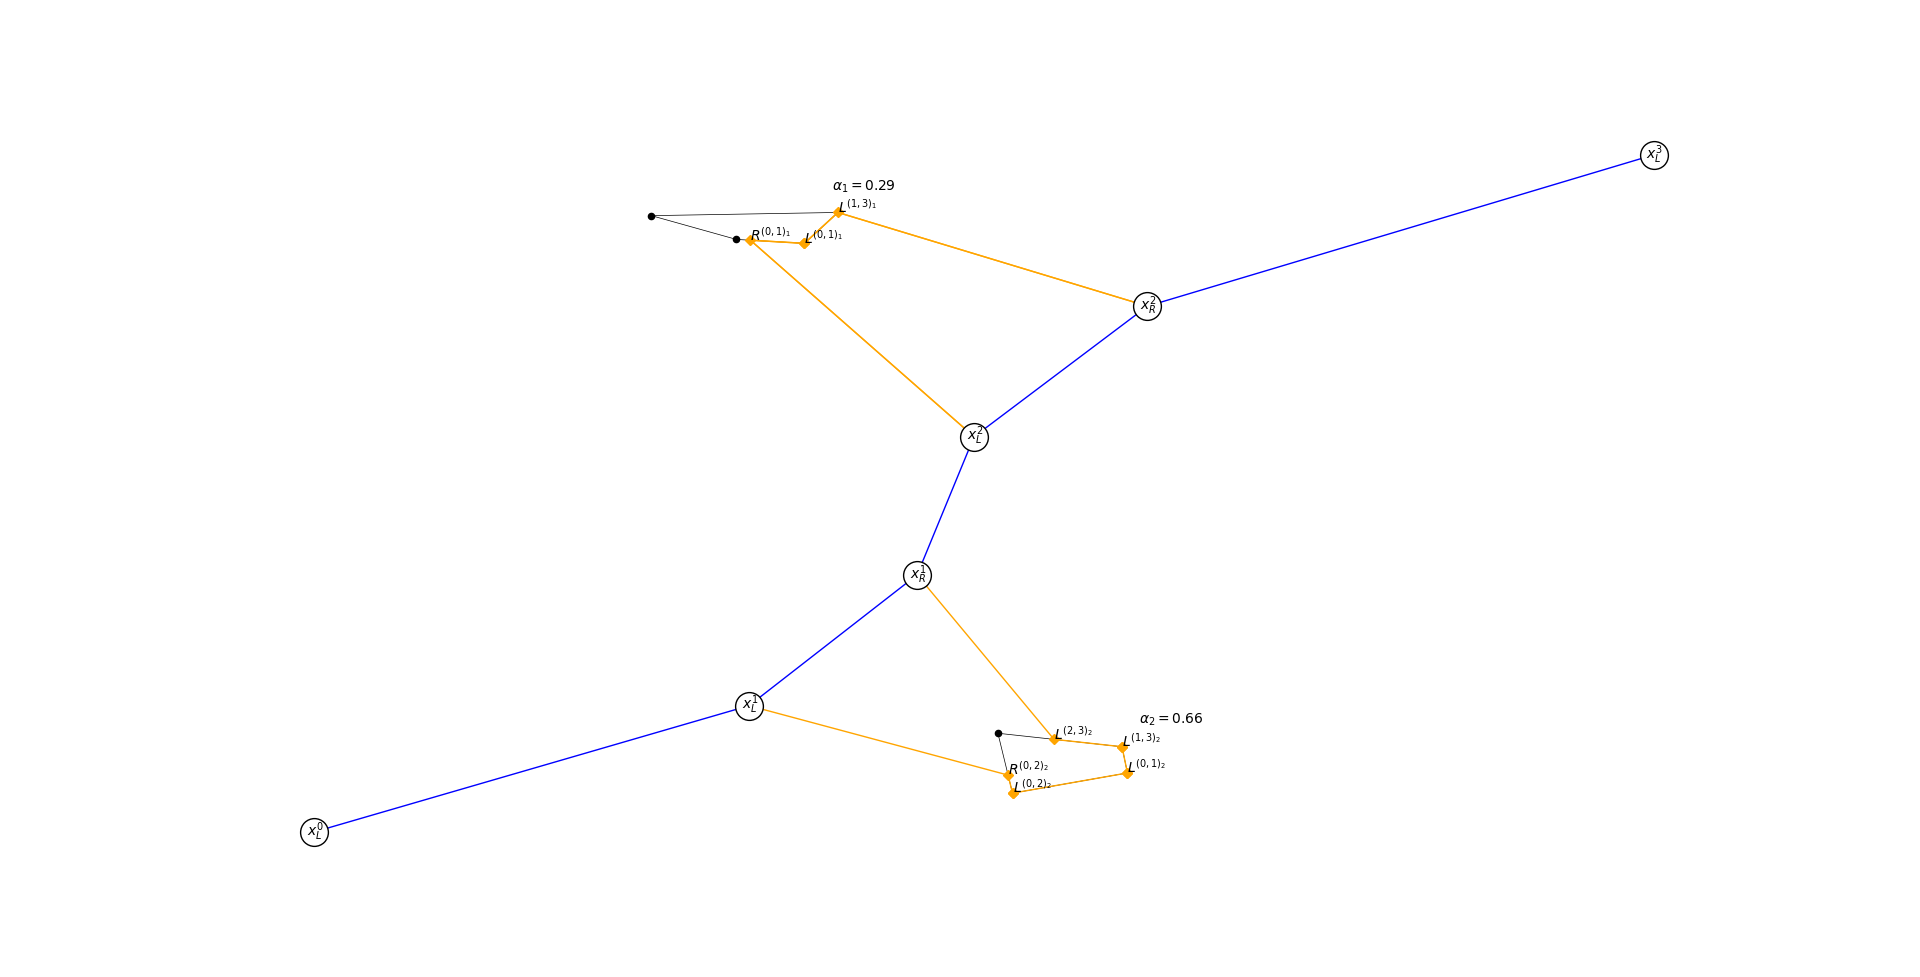
\includegraphics[height=9cm,width=\textwidth]{AMDRPG2.png}
\caption{Example illustrating the meaning of the launching  (L) and rendezvous (R)  points. \label{fig:illustrative}}
\end{figure}

\noindent
Figure \ref{fig:illustrative} shows an example of a configuration with two target graphs with four nodes and four edges. 
The mothership begins at its starting point $x_L^0$. Then, it moves to $x_L^1$ where the drone is launched to visit the graph 2. There, the drone follows a route that ensures the coverage of $66 \%$ of the entire graph and returns to the point $x_R^2$ from where it is launched again to visit the second graph. Once, this graph is visited the drone returns to the mothership at the rendezvous point $x_R^2$ and so on.\\
\noindent
In this formulation of \AMD\xspace the goal is again to find a feasible solution that minimizes the total distance traveled by the drone and the mothership but without using stages. Instead the model ensures the Hamiltonian nature of the routes using the rationale of connectivity by the MTZ or SEC family of constraints.\\
\noindent
Again, we need to be sure that the time spent by the drone to visit the graph $g$ is less than or equal to the time that the mothership needs to move from the launching point to the rendezvous point associated to this graph $g$. Hence, by using the same argument, as the one used in \eqref{DCW-t}, we define for each $g\in \mathcal G$:
\begin{equation}
 \left(\sum_{e_g\in E_g} u^{e_g}d_L^{e_g} + \sum_{e_g, e^\prime_g\in E_g}z^{e_ge^\prime_g}d^{e_ge^\prime_g} + \sum_{e_g\in E_g} \mu^{e_g} d^{e_g} + \sum_{e_g\in E_g}v^{e_g}d_R^{e_g}\right)/v_D\leq d_{RL}^{g}/v_M, \quad\forall g\in\mathcal G.\label{DCW-g}\tag{DCW-g}
\end{equation}

\noindent
Therefore, modifying the previous formulation (AMDRPG-ST), replacing constraints based on stages, one obtains the following alternative valid formulation.
\begin{mini*}|s|
 {}{\sum_{g\in\mathcal G}\sum_{e_g\in E_g} (u^{e_g}d_L^{e_g} + v^{e_g}d_R^{e_g}) + \sum_{g\in\mathcal G}\sum_{e_g\in E_g} \mu^{e_g} d^{e_g} + \sum_{g\in\mathcal G}\sum_{e_g,e^\prime_g\in E_g}z^{e_ge^\prime_g}d^{e_ge^\prime_g} + \sum_{g\in\mathcal G} d_{LR}^g + \sum_{g,g'\in \mathcal G}d_{RL}^{gg'}w^{gg'}}{}{}\label{AMDRPG-MTZ}\tag{AMDRPG-MTZ}
 \addConstraint{\eqref{DEnt2}-\eqref{DInv2}}{}{}
 \addConstraint{\eqref{TOrig}-\eqref{TEnt}}{}{}
 \addConstraint{\eqref{MTZ1} - \eqref{MTZ2} \text{ or } \eqref{SEC} }{}{}
%\addConstraint{\eqref{MTZ3} - \eqref{MTZ6} \text{ or } \eqref{SEC} }{}{}
 \addConstraint{\eqref{MTZ3} - \eqref{MTZ6}}{}{}
 \addConstraint{\eqref{eq:alpha-E} \text{ or } \eqref{eq:alpha-G}}{}{}
 \addConstraint{\eqref{DCW-g}}{}{}
 \addConstraint{\|x_L^g- R^{e_g}\|}{\leq d_L^{e_g},\quad}{\forall e_g:g\in\mathcal G}{}
 \addConstraint{\|R^{e_g}- L^{e_g}\|}{\leq d^{e_g},\quad}{\forall e_g:g\in\mathcal G}{}
 \addConstraint{\|R^{e_g}- L^{e^\prime_g}\|}{\leq d^{e_ge^\prime_g},\quad}{\forall e_g\neq e'_g:g\in\mathcal G}{}
 \addConstraint{\|L^{e_g}- x_R^g\|}{\leq d_R^{e_g},\quad}{\forall e_g:g\in\mathcal G}{}
 \addConstraint{\|x_R^g- x_L^{g'}\|}{\leq d^{gg'}_{RL},\quad}{\forall g,g'\in\mathcal G}{}
 \addConstraint{\|x_L^g- x_R^g\|}{\leq d^g_{LR},\quad}{\forall g\in\mathcal G}{}
 \addConstraint{x_L^0}{= orig}{}
 \addConstraint{x_R^0}{= orig}{}
 \addConstraint{x_L^{|\mathcal G|+1}}{= dest}{}
 \addConstraint{x_R^{|\mathcal G|+1}}{= dest.}{}
\end{mini*}

\noindent
The formulation above \eqref{AMDRPG-MTZ} can be slightly modified replacing constraints $\eqref{MTZ3} - \eqref{MTZ6}$ by
\begin{equation}\label{SEC-graph}
\sum_{g,g'\in \mathcal G} w^{gg'} \le |S|-1, \quad \forall S\subseteq \{1,\ldots, |\mathcal G|\}.
\end{equation}
In doing so we obtain another formulation for \AMD\xspace using SEC rather than MTZ constraints to represent the mothership tour. We will call this formulation (AMDRPG-SEC). Later, we will compare their performance in the computational results section.

\subsubsection{Comparing the formulations\label{ss:compare}}
\noindent
A straightforward analysis of the two types of formulations, namely by stages and based on connectivity, shows that \eqref{AMDRPG-MTZ} has much less variables and constraints than \eqref{AMDRPG-ST}. Indeed, the latter requires definition of distance variables for each $e_g$ and $t$ which is a quadratic function rather than a linear one as used by the former. In addition, to enforce coordination \eqref{AMDRPG-ST} needs constraints (DCW) for each $g\in \mathcal{G},\ t\in T$ whereas \eqref{AMDRPG-MTZ} only uses (DCW) constraints for $g\in \mathcal{G}$. This is an important decrease in the dimension of the problems to be solved. This observation is confirmed in efficiency in problem solving discussed in the experimental results section.


\subsection{Network Mothership-Drone Routing Problem on a Polygonal with Graphs (\PMD)}
\noindent
The most significant difference between \AMD\xspace and  \PMD\xspace is that, in the latter, the mothership cannot move freely in $\mathbb R^2$ but it has to move on a network that models a road system where the mothership (truck) is constrained to move. An intermediate situation between moving freely and moving on a general road network is to assume that the mothership moves on a closed polygonal, namely a piecewise linear, chain. Modeling this situation is a transition step to achieve the more general case of the mothership moving on general networks. We will present the formulations for the \PMD\xspace  following a scheme similar to that of \AMD. First, we present a model by stages and then another one based on connectivity constraints.\\
\noindent
Let $\mathcal P$ denote a polygonal chain parametrized by its breakpoints $V^1, \ldots, V^p$ ordered in the direction of travel. Observe that we are assuming that there exists a pre-specified orientation that determines the direction of the mothership's displacement. Let also $\gamma_L^{et}$ and $\gamma_R^{et}$ be the parameter values that define the points $x_L^t$ and $x_R^t$ on the edge $e$ on $\mathcal P$, respectively. Figure \ref{fig:ex1} illustrates the meaning of the parameters $\gamma_L^{et}$ and $\gamma_R^{et}$ on a polygonal chain with 4 pieces. Then, the distance measured on the polygonal can be obtained by the following expressions for each $t\in T$:
\begin{equation}\tag{$d^{t\mathcal P}_{LR}$}\label{eq:dLRPt}
d_{LR}^{ee't} = \left\{\begin{matrix}
|\gamma_R^{et} - \gamma_L^{et}|\mathcal L(e), & \text{if } e = e',\\
(1 - \gamma_L^{et})\mathcal L(e) + \sum_{e'' = e+1}^{e'-1}\mathcal L(e'') + \gamma_{R}^{e't}\mathcal L(e'), & \text{if } e < e', \\
\gamma_L^{et}\mathcal L(e) + \sum_{e'' = e'+1}^{e-1}\mathcal L(e'') + (1-\gamma_{R}^{e't})\mathcal L(e'), & \text{if } e > e'.
\end{matrix}\right.
\end{equation}

\begin{equation}\tag{$d^{t\mathcal P}_{RL}$}\label{eq:dRLPt}
d_{RL}^{ee't} = \left\{\begin{matrix}
|\gamma_{L}^{et+1}-\gamma_R^{et}|\mathcal L(e), & \text{if } e = e',\\
(1 - \gamma_R^{et})\mathcal L(e) + \sum_{e'' = e+1}^{e'-1}\mathcal L(e'') + \gamma_{L}^{e't+1}\mathcal L(e'), & \text{if } e < e',\\
\gamma_R^{et}\mathcal L(e) + \sum_{e'' = e'+1}^{e-1}\mathcal L(e'') + (1-\gamma_{L}^{e't+1})\mathcal L(e'), & \text{if } e > e'.\\
\end{matrix}\right.
\end{equation}

%\begin{equation}\tag{$d^{t\mathcal P}_{RL}$}\label{eq:dRLPt}
%d_{RL}^{ee't} = \left\{\begin{matrix}
%(\gamma_{L}^{et+1}-\gamma_R^{et})\mathcal L(e), & \text{if } e = e',\\
%(1 - \gamma_R^{et})\mathcal L(e) + \sum_{e'' = e+1}^{e'-1}\mathcal L(e'') + 
%\gamma_{L}^{e't+1}\mathcal L(e')), & \text{if } e < e'.
%\end{matrix}\right.
%\end{equation}
\noindent
This distance requires a binary variable $z_{LR}^{ee't}$ that determines whether $d_{LR}^{ee'}$ is defined by the first or the second expression in the formula:
$$z_{LR}^{ee't} = 1 \text{ if } \mu_{L}^{et} = 1 \text{ and }\mu_{R}^{e't} = 1,$$

\noindent where $\mu_{L}^{et}$ and $\mu_{R}^{et}$ are indicator variables that attain the value one if the launching point (resp. rendezvous point) is placed in the segment $e$ of $\mathcal P$ at the stage $t$.\\
\noindent
Similarly, we define $z_{RL}^{ee't}$:
$$z_{RL}^{ee't} = 1 \text{ if } \mu_{R}^{et} = 1 \text{ and }\mu_{L}^{e't+1} = 1.$$


\begin{figure}[h!]
\begin{center}
 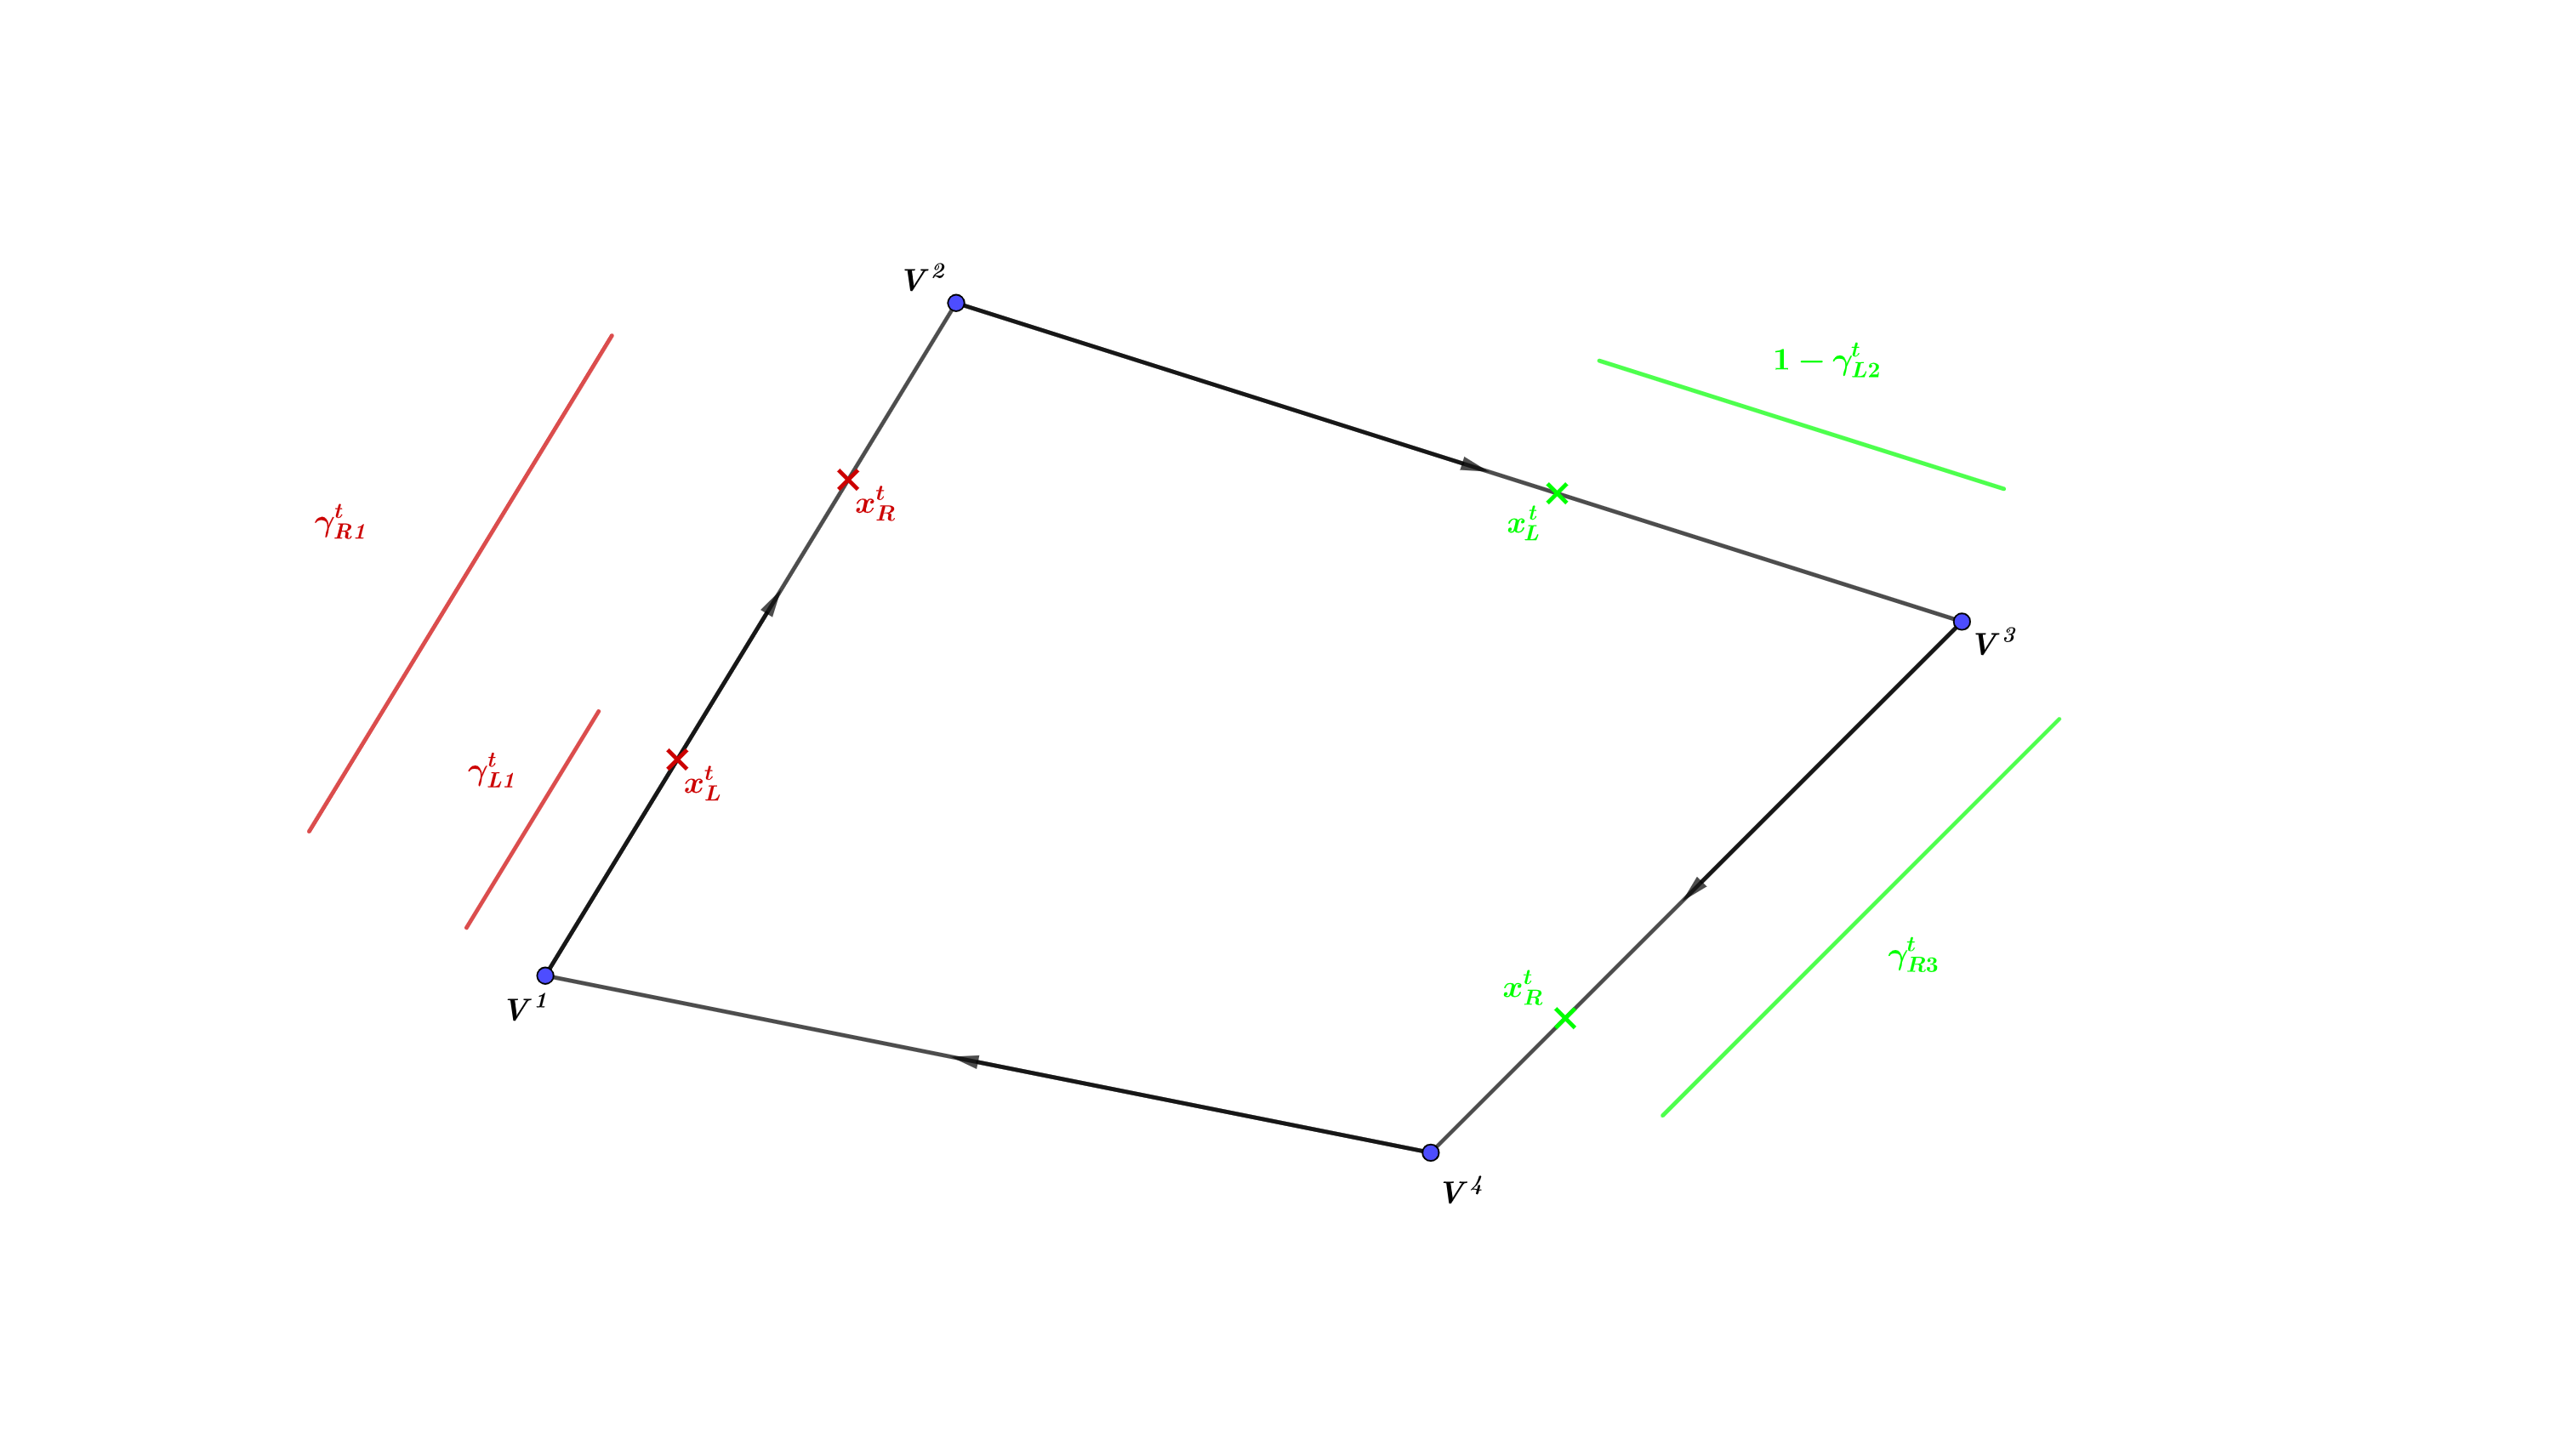
\includegraphics[width=1\linewidth]{PMDRPG.png}
\end{center}
\caption{An example of a parameterization of a mothership route that goes from $V^1$ to $x_L^t$ to launching the drone, then moves to $x_R^t$ on the edge $\overline{V^1V^2}$ to retrieve it, then it goes to $x_L^t$ on $\overline{V^2V^3}$ to launch it again, and travels until $x_R^t$ on $\overline{V^3V^4}$ to retrieve the drone and returns to the starting point at $V^1$.\label{fig:ex1}}
\end{figure}
\noindent
With all this, we can model the movement of the mothership on the polygonal. For each stage $t\in T$, we have

\begin{align}
    x_L^t & = \sum_{e=(i, i+1)\in\mathcal P} \mu_{L}^{et}\left[V^i + \gamma_L^{et}(V^{i+1} - V^i)\right]\label{param1}\\
    x_R^t & = \sum_{e=(i, i+1)\in\mathcal P} \mu_{R}^{et}\left[ V^i + \gamma_R^{et}(V^{i+1} - V^i)\right]\label{param2}\\
    z_{LR}^{ee't} & = \mu_{L}^{et}\mu_{R}^{e't}\label{pol:prodLR}\\
    z_{RL}^{ee't} & = \mu_{R}^{et}\mu_{L}^{e't+1}\label{pol:prodRL}\\
    \sum_{e} \mu_{L}^{et} & = 1  \label{muL} \\
    \sum_{e} \mu_{R}^{et} & = 1 \label{muR}\\
    d_{LR}^t & = \sum_{e, e'} z_{LR}^{ee't} d_{LR}^{ee'} \label{pol:dLRt},\\
    d_{RL}^t & = \sum_{e, e'} z_{RL}^{ee't} d_{RL}^{ee't} \label{pol:dRLt},
\end{align}

\noindent where $d_{LR}^{ee'}$ and $d_{RL}^{ee't}$ are defined in \eqref{eq:dLRPt} and \eqref{eq:dRLPt}. Constraints \eqref{param1} and \eqref{param2} parameterize the launching and rendezvous points on the polygonal chain. Constraints \eqref{pol:prodLR} and \eqref{pol:prodRL} model the product of binary variables. Constraints \eqref{muL} and \eqref{muR} state that, in each stage, the launching and rendezvous points can be only in one segment, not necessarily the same. Constraints \eqref{pol:dLRt} and \eqref{pol:dRLt} compute the total distance between the launching and the rendezvous points in each stage.

\noindent
In addition, for each stage $t\in T$ we can define continuous variables $\lambda_R^t$ and $\lambda_L^t$ that model the absolute position of the point $x_L^t$ in the polygonal to ensure that the movement of the mothership goes always in the allowed direction of travel and never comes back when it traverses the polygonal chain.

\begin{align}
\lambda_L^t - i & \geq \mu_{L}^{et} - (p-1)(1-\mu_{L}^{et}), \quad \forall e=(i, i+1)\in\mathcal P \label{lambdaLg}\\
\lambda_L^t - i & \leq \mu_{L}^{et} - (p-1)(1-\mu_{L}^{et}), \quad \forall e=(i, i+1)\in\mathcal P \label{lambdaLl}\\
\lambda_R^t - i & \geq \mu_{R}^{et} - (p-1)(1-\mu_{R}^{et}), \quad \forall e=(i, i+1)\in\mathcal P \label{lambdaRg}\\
\lambda_R^t - i & \leq \mu_{R}^{et} + (p-1)(1-\mu_{R}^{et}), \quad \forall e=(i, i+1)\in\mathcal P \label{lambdaRl}\\
\lambda_R^t & \geq \lambda_L^t \label{lambdaRL}\\
\lambda_L^{t+1} & \geq \lambda_R^t \label{lambdaLR}
\end{align}

\noindent
Inequalities \eqref{lambdaLg}-\eqref{lambdaRl} link $\mu_{L}^{et}$ and $\lambda_L^t$ (resp. $\mu_{R}^{et}$ and $\lambda_R^t$). Finally, constraints \eqref{lambdaRL} and \eqref{lambdaLR} ensure that the mothership moves in the right direction on the polygonal. \\
% Note that, in this case, it is not required to account for the distance $d_{RL}^t$ because by the assumptions on the model the mothership will traverse all the polygonal chain (since we have imposed that the route starts and ends at the same point).
\noindent
The goal of the (\PMD) is, once again, to find a feasible solution that minimizes the total distance covered by the mothership and the drone. Thus, gathering all the above constraints one gets the following valid formulation.
\begin{mini*}|s|
 {}{\sum_{g\in\mathcal G}\sum_{e_g\in E_g}\sum_{t\in T} (u^{e_gt}d_L^{e_gt} + v^{e_gt}d_R^{e_gt}) + \sum_{g\in\mathcal G}\sum_{e_g\in E_g} \mu^{e_g}d^{e_g} + \sum_{g\in\mathcal G}\sum_{e_g,e^\prime_g\in E_g}z^{e_ge^\prime_g}d^{e_ge^\prime_g} + \sum_{t\in T} (d_{RL}^t + d_{LR}^t)}{}{}\tag{PMDRPG}
 \addConstraint{\eqref{st:DEnt}-\eqref{st:DInv}}{}{}
 \addConstraint{\eqref{param1}-\eqref{pol:dRLt}}{}{}
 \addConstraint{\eqref{MTZ1} - \eqref{MTZ2} \text{ or } \eqref{SEC} }{}{}
 \addConstraint{\eqref{eq:alpha-E} \text{ or } \eqref{eq:alpha-G}}{}{}
 \addConstraint{\eqref{DCW-t}}{}{}
 \addConstraint{\eqref{eq:dLRPt}, \eqref{eq:dRLPt}}{}{}
 \addConstraint{\|x_L^t- R^{e_g}\|}{\leq d_L^{e_gt},\quad}{\forall e_g:g\in\mathcal G,\forall t\in T}{}
 \addConstraint{\|R^{e_g}- L^{e_g}\|}{\leq d^{e_g},\quad}{\forall e_g:g\in\mathcal G,\forall t\in T}{}
 \addConstraint{\|R^{e_g}- L^{e^\prime_g}\|}{\leq d^{e_ge^\prime_g},\quad}{\forall e_g, e'_g:g\in\mathcal G}{}
 \addConstraint{\|L^{e_g}- x_R^t\|}{\leq d_R^{e_gt},\quad}{\forall e_g:g\in\mathcal G,\forall t\in T}{}
%  \addConstraint{\hspace*{-1.5cm} \left(\sum_{e_g\in E_g} u^{e_gt}d_L^{e_gt} + \sum_{e_g, e^\prime_g\in E_g}z^{e_ge^\prime_g}d^{e_ge^\prime_g} + \sum_{e_g\in E_g} \mu^{e_g}d^{e_g} + \sum_{e_g\in E_g} v^{e_gt}d_R^{e_gt}\right)/v_D}{\leq d_{RL}^t/v_M + M(1 - \sum_{e_g\in E_g} u^{e_gt}), \,}{\forall g, t}{}\label{ACW}\tag{{\scriptsize DCW}}
 \addConstraint{x_L^0}{= orig}{}
 \addConstraint{x_R^0}{= orig}{}
 \addConstraint{x_L^{|\mathcal G|+1}}{= dest}{}
 \addConstraint{x_R^{|\mathcal G|+1}}{= dest.}{}
\end{mini*}
\subsubsection{Alternative formulation for \PMD \  based on MTZ-constraints}
\noindent
Analogously to the case of \AMD\xspace one can also model \PMD\xspace without any explicit reference to stages. Here, we will follow a very similar approach to that in Section \ref{sec:AMDMTZ} to describe the formulation for \PMD \ based on MTZ-constraints.\\
\noindent
Let $\mathcal P$ denote, as before,  the polygonal chain parameterized by its endpoints $V^1, \ldots, V^p$ ordered in the direction of travel. In addition, let also $\gamma_{L}^{eg}$ and $\gamma_{R}^{eg}$ be the parameter values that define the points $x_L^g$ and $x_R^g$ on the line segment $\overline{V^iV^{i+1}}$ in $\mathcal P$, respectively. Then, the distance traveled on the polygonal can be obtained by one of  the following expressions. The first one refers to distances covered by the mothership between the launching and rendezvous points of a drone operation, whereas models the distance traveled by the mothership between the launching and rendezvous points of two consecutive graphs targeted in its route.
\begin{equation}\tag{$d_{LR}^{g\mathcal P}$}\label{eq:dLRPg}
d_{LR}^{ee'g} = \left\{\begin{matrix}
|\gamma_{L}^{eg} - \gamma_{R}^{eg}|\mathcal L(e), & \text{if } e = e',\\
(1 - \gamma_{L}^{eg})\mathcal L(e) + \sum_{e'' =e+1}^{e'-1}\mathcal L(e'') + \gamma_{R}^{e'g}\mathcal L(e'), & \text{if } e < e', \\
\gamma_{L}^{eg}\mathcal L(e) + \sum_{e'' = e+1}^{e'-1}\mathcal L(e'') + (1-\gamma_{R}^{e'g})\mathcal L(e'), & \text{if } e > e'.
\end{matrix}\right.
\end{equation}

\begin{equation}\tag{$d_{RL}^{g\mathcal P}$}\label{eq:dRLPg}
d_{RL}^{ee'gg'} = \left\{\begin{matrix}
|\gamma_{L}^{eg} - \gamma_{R}^{eg'}|\mathcal L(e), & \text{if } e = e',\\
(1 - \gamma_{R}^{eg})\mathcal L(e) + \sum_{e'' = e+1}^{e'-1}\mathcal L(e'') + \gamma_{L}^{e'g'}\mathcal L(e'), & \text{if } e < e',\\
\gamma_{R}^{eg}\mathcal L(e) + \sum_{e'' = e+1}^{e'-1}\mathcal L(e'') + (1-\gamma_{L}^{e'g'})\mathcal L(e'), & \text{if } e > e'.
\end{matrix}\right.
\end{equation}
\noindent
This distance requires binary variables $z_{LR}^{ee'g}$ and $z_{RL}^{ee'gg'}$ that determines which of the expressions in \eqref{eq:dLRPg} and  \eqref{eq:dRLPg} define $d_{LR}^{ee'g}$ and $d_{RL}^{ee'gg'}$, respectively.
$$z_{LR}^{ee'g} = 1 \text{ iff } \mu_{L}^{eg} = 1 \text{ and }\mu_{R}^{e'g} = 1,\qquad
z_{RL}^{ee'gg'} = 1 \text{ iff } \mu_{L}^{eg} = 1 \text{ and }\mu_{R}^{e'g'} = 1,
$$
where $\mu_{L}^{eg}$ and $\mu_{R}^{eg}$ are indicator variables that attain the value one if the launching point (resp. rendezvous point) associated to the graph $g$ is placed in the segment $\overline{V^iV^{i+1}}$ of the edge $e=(i, i+1) \in \mathcal P$\\.
\noindent
With all this, we can model the movement of the mothership inside the polygonal. Thus, for each $g, g'\in\mathcal G$ we have:

\begin{align}
    x_L^g & = \sum_{e=(i, i+1)\in\mathcal P} \mu_{L}^{eg}\left[V^i + \gamma_L^{eg}(V^{i+1} - V^i)\right]\label{param1g}\\
    x_R^g & = \sum_{e=(i, i+1)\in\mathcal P} \mu_{R}^{eg}\left[ V^i + \gamma_R^{eg}(V^{i+1} - V^i)\right]\label{param2g}\\
    z_{LR}^{ee'g} & = \mu_{L}^{eg}\mu_{R}^{e'g}\label{prodLRg}\\
    z_{RL}^{ee'gg'} & = \mu_{R}^{eg}\mu_{L}^{e'g'}\label{prodRLg}\\
    \sum_{e} \mu_{L}^{eg} & = 1  \label{muLg} \\
    \sum_{e} \mu_{R}^{eg} & = 1 \label{muRg}\\
    d_{LR}^{g} & = \sum_{e, e'} z_{LR}^{ee'g} d_{LR}^{ee'g} \label{dLRg},\\
    d_{RL}^{gg'} & = \sum_{e, e'} z_{RL}^{ee'gg'} d_{RL}^{ee'gg'} \label{dRLgg},
\end{align}

\noindent where $d_{LR}^g$ and $d_{RL}^{gg'}$ are defined in \eqref{eq:dLRPg} and \eqref{eq:dRLPg}, respectively. Constraints \eqref{param1g} and \eqref{param2g} parameterize the launching and rendezvous points on the polygonal chain. Constraints \eqref{prodLRg} and \eqref{prodRLg} model the product of binary variables. Constraints \eqref{muLg} and \eqref{muRg} state that, in each stage, the launching and rendezvous points can be only in one segment, not necessarily the same. Constraints \eqref{dLRg} and \eqref{dRLgg} compute the total distance between the launching and the rendezvous points for each pair of points. The reader may note that the above representation is similar to that given by \eqref{param1}-\eqref{pol:dRLt} with the exception that in \eqref{param1g}-\eqref{dRLgg} constraints are indexed in the set of graphs $g\in \mathcal{G}$ instead that on the stages. This allows a remarkable reduction in the number of distance variables and constraints as already discussed in Section \ref{ss:compare}.\\
\noindent
The goal of the (\PMD) is to find a feasible solution that minimizes the total distance covered by the drone and the mothership, i.e.,
\begin{mini*}|s|
 {}{\sum_{g\in\mathcal G}\sum_{e_g\in E_g} (u^{e_g}d_L^{e_g} + v^{e_g}d_R^{e_g}) + \sum_{g\in\mathcal G}\sum_{e_g\in E_g} \mu^{e_g}d^{e_g} + \sum_{g\in\mathcal G}\sum_{e_g,e^\prime_g\in E_g}z^{e_ge^\prime_g}d^{e_ge^\prime_g} + \sum_{g\in\mathcal G} d_{LR}^g + \sum_{g,g'\in \mathcal G}d_{RL}^{gg'}w^{gg'}}{}{}\label{PMDRPG-MTZ}\tag{PMDRPG-MTZ}
 \addConstraint{\eqref{DEnt2}-\eqref{DInv2}}{}{}
 \addConstraint{\eqref{TOrig}-\eqref{TEnt}}{}{}
 \addConstraint{\eqref{MTZ1} - \eqref{MTZ2} \text{ or } \eqref{SEC} }{}{}
 \addConstraint{\eqref{MTZ3} - \eqref{MTZ6} \text{ or } \eqref{SEC} }{}{}
 \addConstraint{\eqref{param1g}-\eqref{dRLgg}}{}{}
 \addConstraint{\eqref{eq:alpha-E} \text{ or } \eqref{eq:alpha-G}}{}{}
\addConstraint{\eqref{DCW-g}}{}{}
  \addConstraint{\eqref{eq:dLRPg}, \eqref{eq:dRLPg}}{}{}
 \addConstraint{\|x_L^g- R^{e_g}\|}{\leq d_L^{e_g},\quad}{\forall e_g:g\in\mathcal G}{}
 \addConstraint{\|R^{e_g}- L^{e_g}\|}{\leq d^{e_g},\quad}{\forall e_g:g\in\mathcal G}{}
 \addConstraint{\|R^{e_g}- L^{e^\prime_g}\|}{\leq d^{e_ge^\prime_g},\quad}{\forall e_g:g\in\mathcal G}{}
 \addConstraint{\|L^{e_g}- x_R^i\|}{\leq d_R^{e_g},\quad}{\forall e_g:g\in\mathcal G}{}
%  \addConstraint{\left(\sum_{e_g\in E_g} u^{e_g}d_L^{e_g} + \sum_{e_g, e^\prime_g\in E_g}z^{e_ge^\prime_g}d^{e_ge^\prime_g} + \sum_{e_g\in E_g} \mu^{e_g} d^{e_g} + \sum_{e_g\in E_g}v^{e_g}d_R^{e_g}\right)/v_D}{\leq d_{RL}^{g}/v_M, \quad}{\forall g\in\mathcal G}{}\label{DCW-g}\tag{DCW-g}
 \addConstraint{x_L^0}{= orig}{}
 \addConstraint{x_R^0}{= orig}{}
 \addConstraint{x_L^{|\mathcal G|+1}}{= dest}{}
 \addConstraint{x_R^{|\mathcal G|+1}}{= dest.}{}
\end{mini*}
\noindent
The reader may note that the above formulation actually encloses two different ones depending whether it includes constraints \eqref{MTZ1} - \eqref{MTZ2}  or  \eqref{SEC}. However, for the sake of presentation we have preferred to present them in this compact form to reduce the length of the paper.

\subsection{Network Mothership-Drone Routing Problem with Graphs (\NMD)}
\noindent
This new model is a refinement of the last one as here the mothership has to move on a general undirected network rather than on a polygonal chain.
Even though the previous one, namely \PMD, can be seen as a particular case of \NMD, for the sake of presentation, we have preferred to include it first to ease the understanding of the more advanced \NMD \ model.\\
\noindent
As before, we start with an approach that models the problems by stages. Later, we shall extend the analysis using the rationale of connectivity, as already done in the the previous models \AMD\xspace and \PMD.\\
\noindent
Let $\mathcal N=(V, E)$ be the network that models the space of movement for the mothership. For each stage $t\in T:= \{1,\ldots,|\mathcal G|\}$, we assume that the mothership starts and ends in the edge $e=(i,j), \, e'=(i',j')\in E$, respectively. Then, it follows a route from the launching to the rendezvous point and vice versa, determined by a sequence of intermediate points as shown in Figure \ref{fig:NMDRPG}:

\begin{figure}[h!]
\begin{center}
 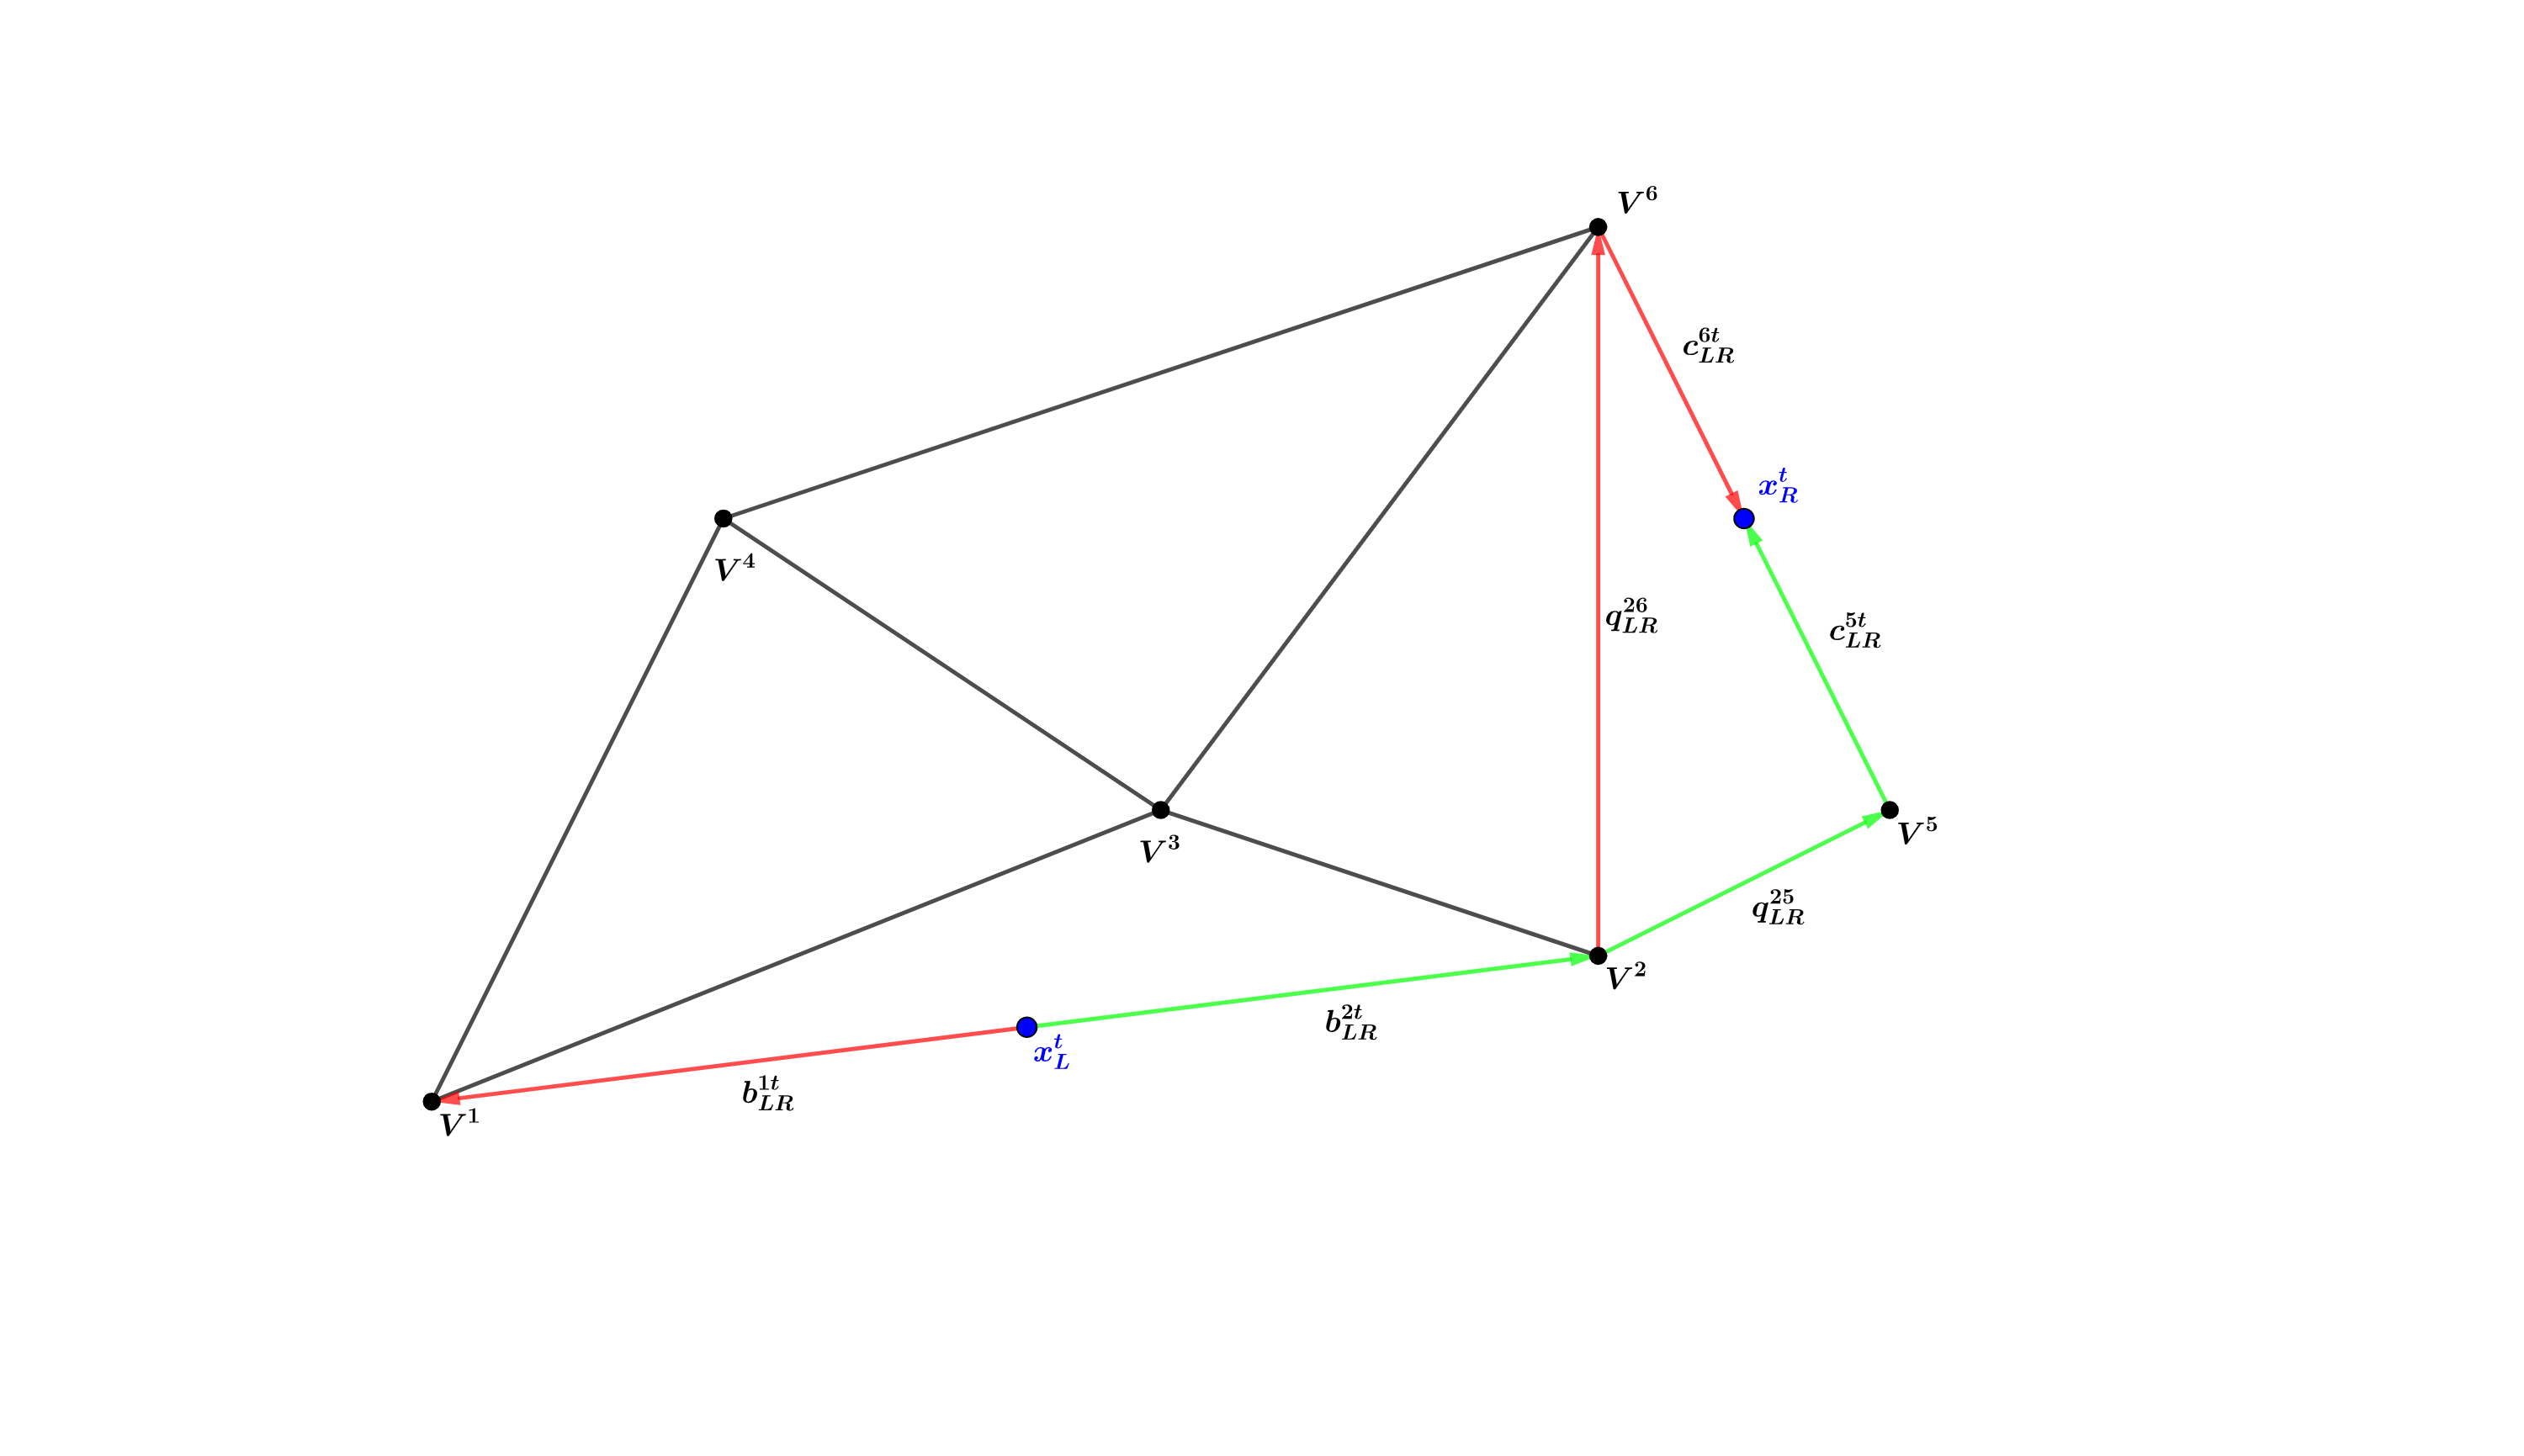
\includegraphics[width=1\linewidth]{NMDRPG.png}
\end{center}
\caption{An example of a parameterization of a mothership route that launches the drone in the point $x_L^t$ on the edge $\overline{V^1V^5}$, then traverses the edge $\overline{V^2V^5}$ and finally moves to $x_R^t$ on the edge $\overline{V^5V^4}$ to retrieve it. The arrows show possible directions of traveling: the green ones are the selected to go from $x_L^t$ to $x_R^t$.}
\label{fig:NMDRPG}
\end{figure}

% $$
% e=(V^i, V^j) \ni x_L^t \rightarrow V^i \vee V^j \rightarrow \ldots \rightarrow V^k \rightarrow \ldots \rightarrow V^{i'} \rightarrow x_R^t \in (V^{i'},V^{j'})=e'.
% $$


% **** \@ Carlos: La notacion de $V_i$ y $i$ es un lio. Esto hay que aclararlo. *****}
\noindent
Therefore, the distance traveled by the mothership, between two consecutive launching and rendezvous points in two edges, not necessarily distinct,  of the graph can be represented as:
\begin{equation}\tag{$d^{t\mathcal N}_{LR}$}\label{eq:dLRNt}
d_{LR}^{ee't} = \left\{\begin{matrix}
|\gamma_{L}^{et} - \gamma_{R}^{et}|\mathcal L(e), & \text{if } e = e',\\
\left[b_{LR}^{it}\gamma_{L}^{et} + b_{LR}^{jt}(1 - \gamma_{L}^{et})\right]\mathcal L(e) + \displaystyle \sum_{e''\in \mathcal N}q_{LR}^{e''t}\mathcal L(e'') + \left[c_{LR}^{i't}\gamma_{R}^{e't} + c_{LR}^{j't}(1 - \gamma_{R}^{e't})\right]\mathcal{L}(e'), & \text{if } e \neq e',
\end{matrix}\right.
\end{equation}

\noindent
where $b_{LR}^{it}$ (resp. $c_{LR}^{it}$) are binary variables that determine from which of the end-points of $e$ (respectively $e'$) one has to account for the distance and $q_{LR}^{et}$ is an integer variable that counts how many times the mothership fully traverses the edge $e$. Furthermore, we need to define another binary variable $z_{LR}^{ee't}$ that models the correct definition of the distance in \eqref{eq:dLRNt}. With the above definition one can account for  the movement of the mothership at each stage $t\in T$ from a launching to a rendezvous  point:

\begin{align}
    x_L^t & = \sum_{e=(i, j)\in E} \mu_{L}^{et}\left[V^i + \gamma_{L}^{et}(V^j - V^i)\right]\label{st:param1bis}\\
    x_R^t & = \sum_{e=(i, j)\in E} \mu_{R}^{et}\left[ V^i + \gamma_{R}^{et}(V^j - V^i)\right]\label{st:param2bis}\\
    z_{LR}^{ee't} & = \mu_{Le}^t\mu_{Re'}^t,\label{st:prodLRbis}\\
    b_{LR}^{it} & \leq \sum_{e\in\delta(i)}\mu_{L}^{et}, \label{st:bLt1}&\qquad\forall i\in V \\
    c_{LR}^{it} & \leq \sum_{e\in\delta(i)}\mu_{R}^{et}, \label{st:cLt1}&\qquad\forall i\in V\\
    b_{LR}^{it} + b_{LR}^{jt} & \geq \mu_L^{et}, &\qquad \forall e=(i, j)\in E\label{st:bLt2}\\
    c_{LR}^{it} + c_{LR}^{jt} & \geq \mu_R^{et}, &\qquad \forall e=(i, j)\in E\label{st:cLt2}\\
    b_{LR}^{it} + \sum_{\{j:(i, j)\in E\}} q_{LR}^{jit} & = \sum_{\{j:(i, j)\in E\}} q_{LR}^{ijt} +  c_{LR}^{it}, \label{st:flow}&\qquad \forall i \in V\\
    \sum_{e\in E} \mu_{L}^{et} & = 1,  \label{st:muLe} \\
    \sum_{e\in E} \mu_{R}^{et} & = 1, \label{st:muRe}\\
    d_{LR}^t & = \sum_{e, e'\in E} z_{LR}^{ee't} d_{LR}^{ee't}, \label{st:dLRt}
\end{align}
\noindent
Constraints \eqref{st:param1bis} and \eqref{st:param2bis} parameterize the launching and rendezvous points in the network $\mathcal N$ at stage $t$. Constraints \eqref{st:prodLRbis} model the product of binary variables. Constraints \eqref{st:bLt1} and \eqref{st:cLt1} state that if the launching point (resp. rendezvous point) is not in the edge $e$, the mothership cannot go (resp. exit) to the vertex that is incident to $e$. Constraints \eqref{st:bLt2} state that if the mothership leaves the edge $e$ to go to $e'$, it must exit from one of the incident vertices to $e$. In the same way, constraints \eqref{st:cLt2} express that if the mothership leaves the edge $e'$ to go to $e$, it must enter to the edge $e$ from one of its incident vertices. Flow conservation constraints \eqref{st:flow} ensure that the number of incoming edges to each vertex $i$ is equal to the number of outgoing edges in the route followed by the mothership. Constraints \eqref{st:muLe} and \eqref{st:muRe} state that, in each stage, the selected points can be only in one edge. Finally, constraints \eqref{st:dLRt} define the total distance between the launching and the rendezvous points at  stage $t$.

\medskip
\noindent
Similarly, the distance covered by the mothership along the path on the network from the rendezvous point $x_R^t$ to the next launching point $x_L^{t+1}$ can be modeled using the following definition of distance:

\begin{equation}\tag{$d^{t\mathcal N}_{RL}$}\label{eq:dRLNt}
d_{RL}^{ee't} = \left\{\begin{matrix}
|\gamma_{R}^{et} - \gamma_{L}^{et+1}|\mathcal L(e), & \text{if } e = e',\\
\left[b_{RL}^{it}\gamma_{R}^{et} + b_{RL}^{jt}(1 - \gamma_{R}^{et})\right]\mathcal L(e) + \displaystyle \sum_{e''\in \mathcal N}q_{RL}^{e''t}\mathcal L(e'') + \left[c_{RL}^{i't}\gamma_{L}^{e't+1} + c_{RL}^{j't}(1 - \gamma_{L}^{e't+1})\right]\mathcal{L}(e'), & \text{if } e \neq e'.
\end{matrix}\right.
\end{equation}
\noindent
In this case, the binary variable $z_{ee'}^{RLt}$ links the rendezvous point at $t$ with the launching point at $t+1$. Then, we can use a set of constraints similar to those used above and the distance from $x_R^t$ to $x_L^{t+1}$ is:
\begin{align}
    z_{RL}^{ee't} & = \mu_{R}^{et}\mu_{L}^{e't+1},\label{st1:prodRL}\\
    b_{RL}^{it} & \leq \sum_{e\in\delta(i)}\mu_{R}^{et}, \label{st1:bRt1}&\qquad \forall i\in V \\
    c_{RL}^{it} & \leq \sum_{e\in\delta(i)}\mu_{L}^{et}, \label{st1:cRt1}&\qquad \forall e\in\delta(i),\,\forall i\in V\\
    b_{RL}^{it} + b_{RL}^{jt} & \geq \mu_R^{et}, &\qquad \forall e=(i, j)\in E\label{st1:bRt2}\\
    c_{RL}^{it} + c_{RL}^{jt} & \geq \mu_L^{et+1}, &\qquad \forall e=(i, j)\in E\label{st1:cRt2}\\
    b_{RL}^{it} + \sum_{\{j:(i, j)\in E\}} q_{RL}^{jit} & = \sum_{\{j:(i, j)\in E\}} q_{RL}^{ijt} +  c_{RL}^{it}, \label{st1:flow}&\qquad \forall i \in V\\
    \sum_{e\in E} \mu_{L}^{et} & = 1,  \label{st1:muLe} \\
    \sum_{e\in E} \mu_{R}^{et} & = 1, \label{st1:muRe}\\
    d_{RL}^t & = \sum_{e, e'\in E} z_{RL}^{ee't} d_{RL}^{ee't}. \label{st1:dRLtN}
\end{align}
\noindent
Constraints \eqref{st1:prodRL} model the product of binary variables. Constraints \eqref{st1:bRt1} and \eqref{st1:cRt1} state that if the rendezvous point (resp. launching point) is not in the edge $e$, the mothership cannot go (resp. exit) to the end vertices of the edge $e$. Constraints \eqref{st1:bRt2} state that if the mothership leaves the edge $e$, it must exit via one of the end vertices of $e$. In the same way, constraints \eqref{st1:cRt2} state that if the mothership goes to the edge $e$, it necessarily must enter to $e$ from one incident vertex of $e$. Flow conservation constraints \eqref{st1:flow} ensure that in the route followed by the mothership the number of used incoming edges to each vertex $i$ is equal to the number of used outgoing edges. Constraints \eqref{st1:muLe} and \eqref{st1:muRe} state that, in each stage, the selected points can be only in one edge. Constraints \eqref{st1:dRLtN} express the total distance between the rendezvous and the launching points at stage $t$.\\
\noindent
Hence, once the distances inside the graph are set with the above two families of constraints, we can state the mathematical programming formulation of the problem as:

\begin{mini*}|s|
 {}{\sum_{g\in\mathcal G}\sum_{e_g\in E_g}\sum_{t\in T} (u^{e_gt}d_L^{e_gt} + v^{e_gt}d_R^{e_gt}) + \sum_{g\in\mathcal G}\sum_{e_g\in E_g}\mu^{e_g} d^{e_g} + \sum_{g\in\mathcal G}\sum_{e_g,e^\prime_g\in E_g}z^{e_ge^\prime_g}d^{e_ge^\prime_g} + \sum_{t\in T} (d_{RL}^t + d_{LR}^t)}{}{}\tag{NDRPG-ST}
 \addConstraint{\eqref{st:DEnt}-\eqref{st:DInv}}{}{}
 \addConstraint{\eqref{st:param1bis}-\eqref{st1:dRLtN}}{}{}
 \addConstraint{\eqref{MTZ1} - \eqref{MTZ2} \text{ or } \eqref{SEC} }{}{}
 \addConstraint{\eqref{eq:alpha-E} \text{ or } \eqref{eq:alpha-G}}{}{}
 \addConstraint{\eqref{DCW-t}}{}{}
 \addConstraint{\eqref{eq:dLRNt}, \eqref{eq:dRLNt}}{}{}
 \addConstraint{\|x_L^t- R^{e_g}\|}{\leq d_L^{e_gt},\quad}{\forall e_g:g\in\mathcal G,\forall t\in T}{}
 \addConstraint{\|R^{e_g}- L^{e_g}\|}{\leq d_g^{e_g},\quad}{\forall e_g:g\in\mathcal G,\forall t\in T}{}
 \addConstraint{\|R^{e_g}- L^{e^\prime_g}\|}{\leq d^{e_ge^\prime_g},\quad}{\forall e_g:g\in\mathcal G,\forall t\in T}{}
 \addConstraint{\|L^{e_g}- x_R^i\|}{\leq d_R^{e_gt},\quad}{\forall e_g:g\in\mathcal G,\forall t\in T}{}
 \addConstraint{x_L^0}{= orig}{}
 \addConstraint{x_R^0}{= orig}{}
 \addConstraint{x_L^{|\mathcal G|+1}}{= dest}{}
 \addConstraint{x_R^{|\mathcal G|+1}}{= dest.}{}
\end{mini*}
\noindent
Again, the objective function has four terms: the first three compute the distances traveled by the drone, while the last one computes the distances traveled by the mothership. Constraints \eqref{st:DEnt}-\eqref{st:DInv} model the tour made by the drone. Constraints \eqref{st:param1bis}-\eqref{st1:dRLtN} model the path following by the mothership in the graph. The rest of the constraints are similar to those explained in the model \eqref{AMDRPG-ST}.

\subsubsection{MTZ formulation for the Network Mothership-Drone Routing Problem with Graphs}
\noindent
In order to apply this type of constraints to model connectivity of the routes we have to reformulate the expressions for the distances so that they are not related to stages. In this case, we observe that the distance between launching and rendezvous points in two edges $e=(i,j),\, e'=(i',j')\in E$, not necessarily distinct,  of the graph can be represented as:
\begin{equation}\tag{$d^{g\mathcal N}_{LR}$}\label{eq:dLRg}
d_{LR}^{ee'g} = \left\{\begin{matrix}
|\gamma_{L}^{eg} - \gamma_{R}^{eg}|\mathcal L(e), & \text{if } e = e',\\
\left[b_{LR}^{ig}\gamma_{L}^{eg} + b_{LR}^{jg}(1 - \gamma_{L}^{eg})\right]\mathcal L(e) + \displaystyle \sum_{e''\in \mathcal N}q_{LR}^{e''g}\mathcal L(e'') + \left[c_{LR}^{i'g}\gamma_{R}^{e'g} + c_{LR}^{j'g}(1 - \gamma_{R}^{e'g})\right]\mathcal{L}(e'), & \text{if } e \neq e',
\end{matrix}\right.
\end{equation}

\noindent
where $b_{LR}^{ig}$ (resp. $c_{LR}^{ig}$) are binary variables that determine from which of the end-points of $e$ (respectively $e'$) one has to account for the distance and $q_{LR}^{eg}$ is a binary variable that is one when the mothership fully traverses the edge $e$. Furthermore, we need to define binary variables $z_{LR}^{ee'g}$ that model the choice of the model for right definition (first or second formulas in \eqref{eq:dLRg} of the distance in \eqref{eq:dLRg}). All the above arguments give the necessary elements to account for the movement of the mothership on the network $\mathcal{N}=(V,E)$:

\begin{align}
    x_L^g & = \sum_{e=(i, j)\in E} \mu_{L}^{eg}\left[V^i + \gamma_{L}^{eg}(V^j - V^i)\right]\label{g:param1bisg}\\
    x_R^g & = \sum_{e=(i, j)\in E} \mu_{R}^{eg}\left[ V^i + \gamma_{R}^{eg}(V^j - V^i)\right]\label{g:param2bisg}\\
    z_{LR}^{ee'g} & = \mu_{L}^{eg}\mu_{R}^{e'g},\label{g:prodLR}\\
    b_{LR}^{ig} & \leq \sum_{e\in\delta(i)} \mu_{L}^{eg}, \label{g:bLt1}&\qquad \forall i\in V \\
    c_{LR}^{ig} & \leq \sum_{e\in\delta(i)} \mu_{R}^{eg}, \label{g:cLt1}&\qquad \forall i\in V\\
    b_{LR}^{ig} + b_{LR}^{jg} & \geq \mu_L^{eg}, &\qquad \forall e=(i, j)\in E\label{g:bLt2}\\
    c_{LR}^{ig} + c_{LR}^{jg} & \geq \mu_R^{eg}, &\qquad \forall e=(i, j)\in E\label{g:cLt2}\\
    b_{LR}^{ig} + \sum_{\{j:(i, j)\in E\}} q_{LR}^{jig} & = \sum_{\{j:(i, j)\in E\}} q_{LR}^{ijg} +  c_{LR}^{ig}, \label{g:flow}&\qquad \forall i \in V\\
    \sum_{e\in E} \mu_{L}^{eg} & = 1,  \label{g:muLe} \\
    \sum_{e\in E} \mu_{R}^{eg} & = 1, \label{g:muRe}\\
    d_{LR}^g & = \sum_{e, e'\in E} z_{LR}^{ee'g} d_{LR}^{ee'g}, \label{g:dLRgN}
\end{align}
\noindent
Constraints \eqref{g:param1bisg} and \eqref{g:param2bisg} parameterize the launching and rendezvous points in the network $\mathcal N$ induced by the visit to the graph  $g\in \mathcal{G}$. Constraints \eqref{g:prodLR} model the product of binary variables. Constraints \eqref{g:bLt1} and \eqref{g:cLt1} state that if the launching point (resp. rendezvous point) is not in the edge $e$, the mothership cannot go (resp. exit) to the vertices of the edge $e$. Constraints \eqref{g:bLt2} state that if the mothership leaves the edge $e$, it must exit from one of the incident vertices to $e$. In the same way, constraints \eqref{g:cLt2} state that if the mothership leaves the edge $e'$, it necessarily must enter to $e$ from one incident vertex of $e$. Flow conservation constraints \eqref{g:flow} ensure that, in the route to be defined, the number of incoming edges to each vertex $i$ is equal to the number of outgoing edges. Constraints \eqref{g:muLe} and \eqref{g:muRe} state that, for the visit to the graph  $g\in \mathcal{G}$, launching and rendezvous points can be only in one edge. Constraints \eqref{g:dLRgN} returns the total distance traveled by the drone on the graph  $g\in \mathcal{G}$.

\medskip
\noindent
Similarly, the distance covered by the mothership along the path on the network $\mathcal{N}$, from the rendezvous point $x_R^g\in e$, after the visit to $g\in \mathcal{G}$ to the next launching point $x_L^{g'}\in e'$ (to go to the graph $g'\in \mathcal{G}$), can be modeled using the following definition of distance:

\begin{equation}\tag{$d^{g\mathcal N}_{RL}$}\label{eq:dRLg}
d_{RL}^{ee'gg'} = \left\{\begin{matrix}
|\gamma_{R}^{eg} - \gamma_{L}^{eg'}|\mathcal L(e), & \text{if } e = e',\\
\left[b_{RL}^{ig}\gamma_{R}^{eg} + b_{RL}^{jg}(1 - \gamma_{R}^{eg})\right]\mathcal L(e) + \displaystyle \sum_{e''\in \mathcal N}q_{RL}^{e''gg'}\mathcal L(e'') + \left[c_{RL}^{i'g'}\gamma_{L}^{e'g'} + c_{RL}^{j'g'}(1 - \gamma_{L}^{e'g'})\right]\mathcal L(e'), & \text{if } e \neq e'.
\end{matrix}\right.
\end{equation}
\noindent
In this case, the binary variable $z_{RL}^{ee'gg'}$ links the rendezvous point at $g$ with the launching point at $g'$. Then, we can use a set of constraints similar to those used above and the distance from $x_R^g$ to $x_L^{g'}$ is:

\begin{align}
    z_{RL}^{ee'gg'} & = \mu_{R}^{eg}\mu_L^{e'g'},\label{prodRLggN}\\
    b_{RL}^{ig} & \leq \sum_{e\in\delta(i)}\mu_{R}^{eg}, \label{bRt1}&\qquad \forall i\in V \\
    c_{RL}^{ig} & \leq \sum_{e\in\delta(i)}\mu_{L}^{eg}, \label{cRt1}&\qquad \forall i\in V\\
    b_{RL}^{ig} + b_{RL}^{jg} & \geq \mu_R^{eg}, &\qquad \forall e=(i, j)\in E\label{bRt2}\\
    c_{RL}^{ig} + c_{RL}^{jg} & \geq \mu_L^{eg}, &\qquad \forall e=(i, j)\in E\label{cRt2}\\
    b_{RL}^{ig} + \sum_{\{j:(i, j)\in E} q_{RL}^{jigg'} & = \sum_{\{j:(i, j)\in E\}} q_{RL}^{ijgg'} +  c_{RL}^{ig'}, \label{flow}&\qquad \forall i \in V\\
    d_{RL}^{gg'} & = \sum_{e, e'} z_{RL}^{ee'gg'} d_{RL}^{ee'gg'}. \label{dRLt}
\end{align}
\noindent
Hence, once the distances inside the graph are set with the above two families of constraints, we can state the mathematical programming formulation of the problem as:

\begin{mini*}|s|
 {}{\sum_{g\in E_g} (u^{e_g}d_L^{e_g} + v^{e_g}d_R^{e_g}) + \sum_{e_g\in E_g}\mu^{e_g} d^{e_g} + \sum_{e_g,e^\prime_g\in E_g}z^{e_ge^\prime_g}d^{e_ge^\prime_g}+ \sum_{g\in E_g} d_{LR}^g + \sum_{g,g'\in E_g}d_{RL}^{gg'}w^{gg'}}{}{}\tag{NDRPG-MTZ}
 \addConstraint{\eqref{st:DEnt}-\eqref{st:DInv}}{}{}
 \addConstraint{\eqref{g:param1bisg}-\eqref{dRLt}}{}{}
 \addConstraint{\eqref{MTZ1} - \eqref{MTZ2} \text{ or } \eqref{SEC} }{}{}
 \addConstraint{\eqref{eq:alpha-E} \text{ or } \eqref{eq:alpha-G}}{}{}
 \addConstraint{\eqref{DCW-g}}{}{}
 \addConstraint{\eqref{eq:dLRg}, \eqref{eq:dRLg}}{}{}
 \addConstraint{\|x_L^g- R^{e_g}\|}{\leq d_L^{e_g},\quad}{\forall e_g:g\in\mathcal G}{}
 \addConstraint{\|R^{e_g}- L^{e_g}\|}{\leq d_g^{e_g},\quad}{\forall e_g:g\in\mathcal G}{}
 \addConstraint{\|R^{e_g}- L^{e^\prime_g}\|}{\leq d^{e_ge^\prime_g},\quad}{\forall e_g:g\in\mathcal G,e^\prime_g}{}
 \addConstraint{\|L^{e_g}- x_R^g\|}{\leq d_R^{e_g},\quad}{\forall e_g:g\in\mathcal G}{}
 \addConstraint{x_L^0}{= orig}{}
 \addConstraint{x_R^0}{= orig}{}
 \addConstraint{x_L^{|\mathcal G|+1}}{= dest}{}
 \addConstraint{x_R^{|\mathcal G|+1}}{= dest.}{}
\end{mini*}

% $$
% e=(i, j) \ni x_R^t \rightarrow V_i \vee V_j \rightarrow \ldots \rightarrow V_k \rightarrow \ldots \rightarrow V_{i'} \rightarrow x_L^{t+1} \in (i',j')=e'
% $$

% The design of these paths obeys to define binary variables that decide which vertices are selected in each stage $t$: 
\section{Strengthening the formulations of \MDR}\label{bounds}
\noindent
The different models that we have proposed include in one way or another big-M constants. We have defined different big-M constants along this work. In order to strengthen the formulations we provide tight upper and lower bounds for those constants. In this section we present some results that adjust them for each one of the the models.

\subsubsection*{Big $M$ constants bounding the distance from the launching / rendezvous point on the path followed by the mothership to the rendezvous / launching point on the target graph $g\in \mathcal{G}$}
\begin{itemize}
\item \underline{\AMD}. To linearize the first term of the objective function in \AMD, we define the auxiliar non-negative continuous variables $p_L^{e_gt}$ and (resp. $p_R^{e_gt}$) to model the product by including the following constraints:
\begin{align*}
p_L^{e_gt} & \geq m_L^{e_g} u^{e_gt}, \\
p_L^{e_gt} & \leq d_L^{e_g} - M_L^{e_gt}(1-u^{e_gt}).
\end{align*}
The best upper bound $M_R^{e_gt}$ or $M_L^{e_gt}$ that we can consider is the full diameter of the data, that is the maximum distance between every pair of vertices of the graphs $g\in \mathcal{G}$, in input the data, i.e., every launching or rendezvous point is inside the circle whose diametrically opposite points are the explained below. 
$$
M_R^{e_gt} = \max_{\{v\in V_g, v'\in V_{g'} : g, g'\in\mathcal G\}} \|v - v'\| = M_L^{e_gt}.
$$

On the other hand, the minimum distance in this case can be zero. This bound is attainable whenever the launching or the rendezvous points of the mothership is the same that the rendezvous or launching point on the target graph $g\in \mathcal{G}$.

\item \underline{\NMD}. In this case, the best upper bounds for $M_R^{e_gt}$ or $M_L^{e_gt}$ is the maximum distance between the polygonal chain $\mathcal{P}$ or the graph $\mathcal{N}$ and any of the target graphs $g\in \mathcal{G}$:
$$
M_R^{e_gt} = \max_{\{v\in V_g, w\in \mathcal N\}}\|v - w\| = M_L^{i_gt}.
$$
On the other hand, the minimum distance can be computed by taking the closest points between the graph $g$ and the network $\mathcal{N}$:
$$
m_R^{e_gt} = \min_{\{v\in V_g, w\in \mathcal N\}}\|v - w\| = m_L^{e_gt}.
$$
\end{itemize}

\subsubsection*{Bounds on the big $M$ constants for the distance from the launching point to the rendezvous points for the MTZ/SEC formulations in \AMD}

We can compute a tighter upper bound for the distance $d_{RL}^{gg'}$ between each pair of graphs $g,g'$ for the constraints obtained by the linearization of its product:
\begin{align*}
p^{gg'} & \geq m_{RL}^{gg'} d_{RL}^{gg'}, \\
p^{gg'} & \leq d_{RL}^{gg'} - M_{RL}^{gg'}(1-w^{gg'}).
\end{align*}
This upper bound $M_{RL}^{gg'}$ is given by the diameter of $g\cup g'$:
$$
M_{RL}^{gg'} = \max_{\{v\in V_g, v'\in V_{g'}\}}\|v - v'\|.
$$


\subsubsection*{Bounds on the big $M$ constants for the distance from the launching to the rendezvous points on the target graph $e\in \mathcal{G}$.} When the drone visits a graph $g$, it has to go from one edge $e_g$ to another edge $e'_g$ depending on the order given by $z^{e_ge_g'}$. This fact produces another product of variables linearized by the following constraints:
\begin{align*}
p^{e_ge'_g} & \geq m^{e_ge_g'} d_{RL}^{gg'}, \\
p^{e_ge_g'} & \leq d^{e_ge_g'} - M^{e_ge_g'}(1-z^{e_ge_g'}).
\end{align*}

\noindent
Since we are taking into account the distance between two edges $e=(B^{e_g},C^{e_g}) , e'=(B^{e^\prime_g},C^{e^\prime_g})\in E_g$, the maximum and minimum distances between their vertices give us the upper and lower bounds:
\begin{align*}
M^{e_g e^\prime_g} = & \max\{\|B^{e_g} - C^{e^\prime_g}\|, \|B^{e_g} - B^{e^\prime_g}\|, \|C^{e_g} - B^{e^\prime_g}\|, \|C^{e_g} - C^{j_g}\|\}, \\
m^{e_g e^\prime_g} = & \min\{\|B^{e_g} - C^{e^\prime_g}\|, \|B^{e_g} - B^{e^\prime_g}\|, \|C^{e_g} - B^{e^\prime_g}\|, \|C^{e_g} - C^{e^\prime_g}\|\}.
\end{align*}

\subsubsection*{Bounds on the big $M$ constants for the distance covered by the mothership on the polygonal for the \PMD \ model during one drone operation.}
In the case of \PMD, we can also set tighter upper bounds for the distance covered by the drone inside the polygonal during an operation that starts in $e$ and finishes at $e'$ (or vice versa) (see \eqref{pol:dLRt} and \eqref{pol:dRLt}). This is clearly bounded from above by the total length of the line segments where the mothership is located. 
\begin{equation*}
M_{LR}^{ee't} = M_{RL}^{ee't} = \left\{\begin{matrix}
\mathcal L(e), & \text{if } e = e',\\ 
\displaystyle \sum_{e<e''<e'}\mathcal L(e'') & \text{if } e < e', \\
\displaystyle \sum_{e'<e''<e}\mathcal L(e'') & \text{if } e > e'.
\end{matrix}\right.
\end{equation*}


\subsubsection*{Bounds on the big $M$ constants for the distance covered by the drone during an operation for all the models by stages}
To link the drone operation with the mothership travel in the models by stages, we have defined the constraint $\eqref{DCW-t}$ that includes the $M$:
\begin{equation*}
\left(\sum_{e_g\in E_g} u^{e_gt}d_L^{e_gt} + \sum_{e_g, e^\prime_g\in E_g}z^{e_ge^\prime_g}d^{e_ge^\prime_g} + \sum_{e_g\in E_g} \mu^{e_g}d^{e_g} + \sum_{e_g\in E_g} v^{e_gt}d_R^{e_gt}\right)/v_D \leq d_{RL}^t/v_M + M(1 - \sum_{e_g\in E_g} u^{e_gt})
\end{equation*}
\noindent
To obtain this upper bound $M$ we add to the length of the graph $\mathcal L(g)$ the big-Ms computed for $u^{e_gt}$ and $v^{e_gt}$, that is, $M_{L}^{e_gt}$ and $M_R^{e_gt}$, and the maximum distances that can be employed by the drone to move from one edge to another one:

$$M = \mathcal{L}(g) + M_L^{e_gt} + M_R^{e_gt} + \sum_{e_g, e_g'\in E_g}M^{e_ge_g'}.$$


\section{A Matheuristic for the Mothership-Drone Routing Problem with Graphs}\label{Math}
\noindent
This section is devoted to present our matheuristic approach to address the solution of the \MDR. Our motivation comes from the fact that the exact methods presented in the previous section are highly time demanding. Alternatively, the matheuristic provides good quality solution in limited computing times.\\
\noindent
First, we focus on the case in which the mothership can move freely on the continuous space, namely \AMD.
The basic idea of the algorithm is to determine first the sequence of visits to the target graphs in $\mathcal{G}$. This route is obtained replacing each graph in $\mathcal{G}$ by its centroid and then solving a TSP over the neighborhoods of those centroids, namely a XPPN (see \cite{art:Puerto2020}). Then, given such an order of visits, the launching/rendezvous points where the mothership must stop, are determined by solving a \AMD\xspace problem, but limited to one single graph per time, following the sequence previously computed. Successively, the solution so obtained is improved by providing it to the solver as initial partial solution and by solving, once more, another \AMD \ problem, where now we fix the launching/rendezvous points but leave free the variables $w$ that give the sequence of visits to the targets graphs, i.e., without fixing the order of visits.
If the solution so obtained consists in a different order of visit of the graphs with respect to the previous one, the procedure is repeated to generate a new feasible solution. The stopping criterion is to find a solution that does not change with respect to the one obtained in the previous cycle of the algorithm.
In the following, we present the pseudo-code of this algorithm:


\begin{itemize} 
\item[STEP 1] (Centroids of the graphs)\\
- Let $orig$ be the origin/destination of the mothership tour (orange point with label $0$ in Figure \ref{fig:example} [a]).\\
For each graph $g \in \mathcal G$:\\
- identify its centroid $c_g$ and consider its neighborhood defined as the circle $\rho(c_g,2)$ (red points in Figure \ref{fig:example} [a]).
\item[STEP 2] (Order of visit of the graphs)
Determine an order of visit for the graphs in $\mathcal{G}$ by solving the XPPN of the mothership over the set of the neighborhoods associated with the centroids of those graphs (blue tour 0, 1, 2, 3, 4, 0 in Figure  \ref{fig:example} [a]).\\

\item[STEP 3] (launching/rendezvous points location)
Let $\bar{w}_{gg^{'}}, \: \forall g,g^{'} \in \mathcal G$ be the optimal values of the variables $w_{gg^{'}}$ generated by STEP 2.\\
Following this order of visit, set the launching point for the first graph as the depot, then solve the resulting \AMD\xspace limited to the first graph.\\
Repeat the same procedure for the remaining graphs to be visited, by solving \AMD\xspace on one single graph per time, by fixing as launching point of the current graph the rendezvous point of the previous graph.

\item [STEP 4] (Solution update) 
Let $\bar{z}$ be the solution obtained by STEP 3, consisting of the tour of the drone on each target  (Figure \ref{fig:example} [b]), and $\bar{x}_{L}^{g}$, $\bar{x}_{R}^{g} \:\: \forall g \in \mathcal G$ the associated launching/rendezvous points (green and blue points in Figure \ref{fig:example} [b]).\\
Solve the model \AMD\xspace with these launching/rendezvous points but leaving free the $w_{gg^{'}} \:\:\ \forall g,g^{'} \in \mathcal G$ variables and providing to the solver $\bar{z}$ as initial partial solution.
\item [STEP 5]
Let $\hat{z}$ be the updated solution obtained by STEP 4 (again Figure \ref{fig:example} [b] for this illustrative example) and $\hat{w}_{gg^{'}}$ the associated order of visit of the graphs.\\
If the $\hat{w}_{gg^{'}} \neq \bar{w}_{gg^{'}}$ repeat from STEP 3, otherwise stop.
\end{itemize}
\noindent
Note that in the example shown in Figure \ref{fig:example} we solved the \AMD\xspace model by imposing that at least a given percentage of each target must be visited. For this reason the solution consists in drone's missions which visit only part of each graph, as represented by the red segments in Figure \ref{fig:example} [b]. Moreover, for this example, most of the launching/rendezvous points coincide. More precisely, considering Figure \ref{fig:example} [b], the drone starts from the origin and visits part of the first target. The mothership retrieves it at the point labelled 1. From the same point the drone starts the second mission to visit part of the second target and then reaches the mothership at the point labelled 2. From that point the drone starts for visiting the third target meeting the mothership at the point labelled 3. From this latter point the last mission of the drone starts and ends on the mothership at the point labelled 4. Then the mothership with the drone go back to the origin. In this example the solution obtained at STEP 4, by fixing the launching/rendezvous points but not the order of visit, does not change with respect to the one obtained at STEP 3. Thus the procedure stops after the first iteration and provides the solution shown in Figure \ref{fig:example} [b].
The exact resolution of \AMD\xspace can be hard expecially on large instances. For this reason for each call of the solver within the heuristic procedure, we set a maximum number of solutions that the solver can generate before stopping.\\
The procedure adopted for the  \NMD \xspace problem consists in the same steps of the matheuristic presented above for the \AMD \xspace problem but, at STEP 4, the partial solution, given in input to the solver, includes also the values of the variables modelling the routing of the truck on the graph.
%\CV{This procedure is similar for the \NMD  problem by providing, in addition, the variables that model the routing of the truck in the graph as initial partial solution at STEP 4.}


\begin{figure}%
    \centering
    \subfloat[a]{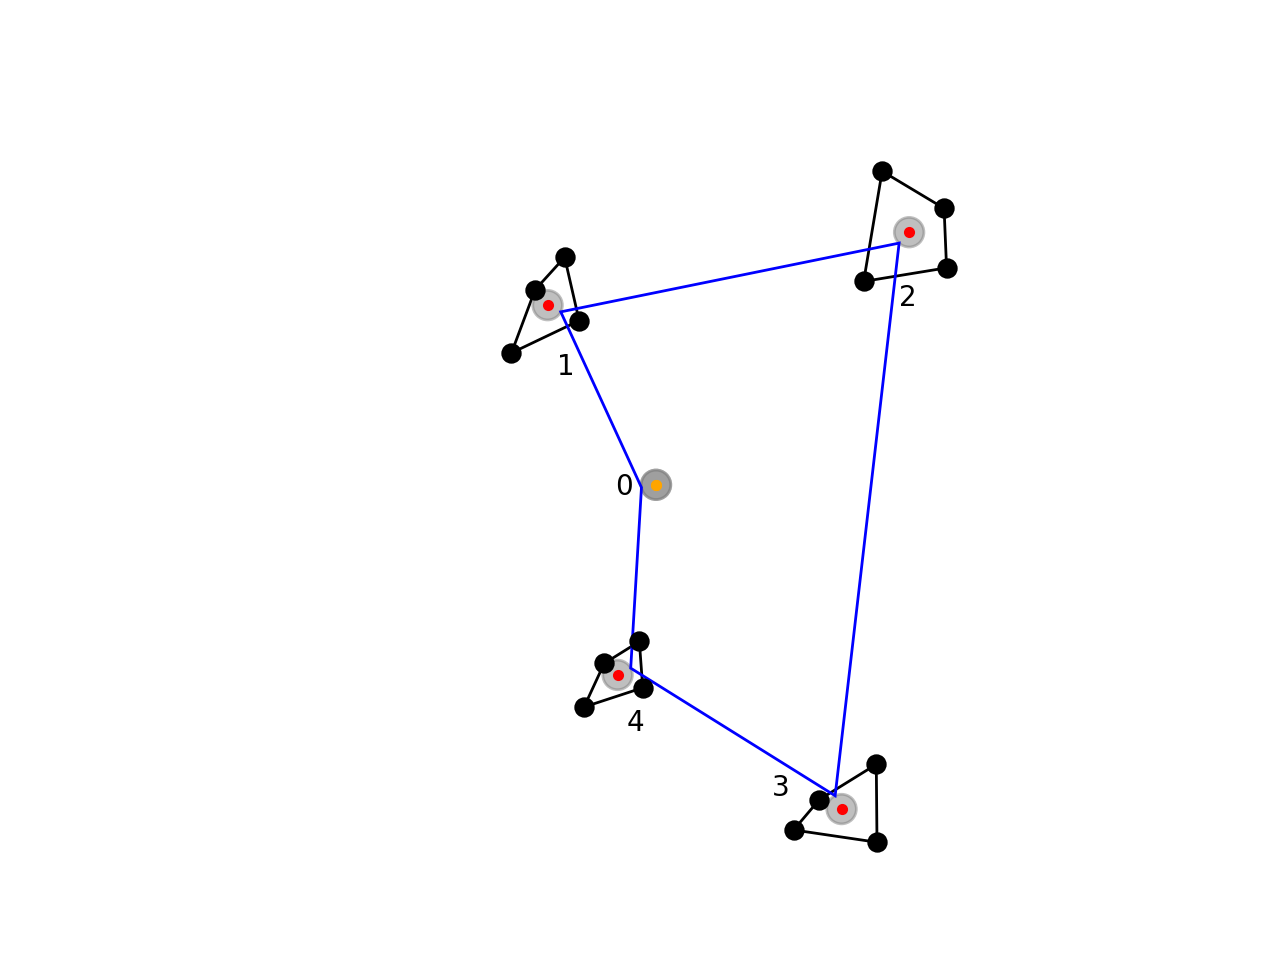
\includegraphics[width=5cm]{./step0.png} }%
    \qquad
    \subfloat[b]{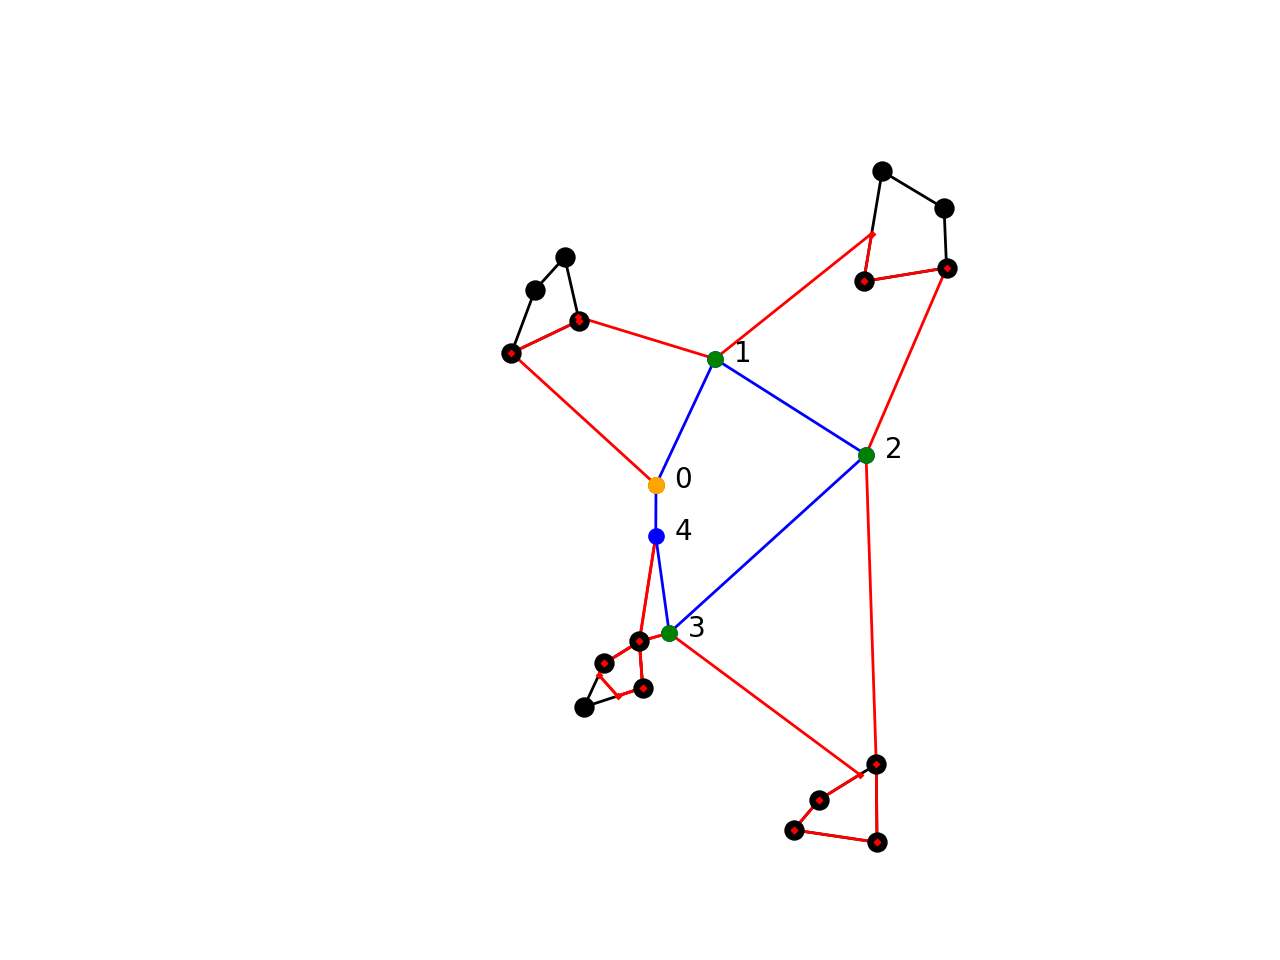
\includegraphics[width=5cm]{./step1.png} }%
    \caption{Illustrative example}%
    \label{fig:example}%
\end{figure}







% \input{Benders-like}
\section{Experimental results}


% \begin{figure}[h!]
% \begin{center}
%  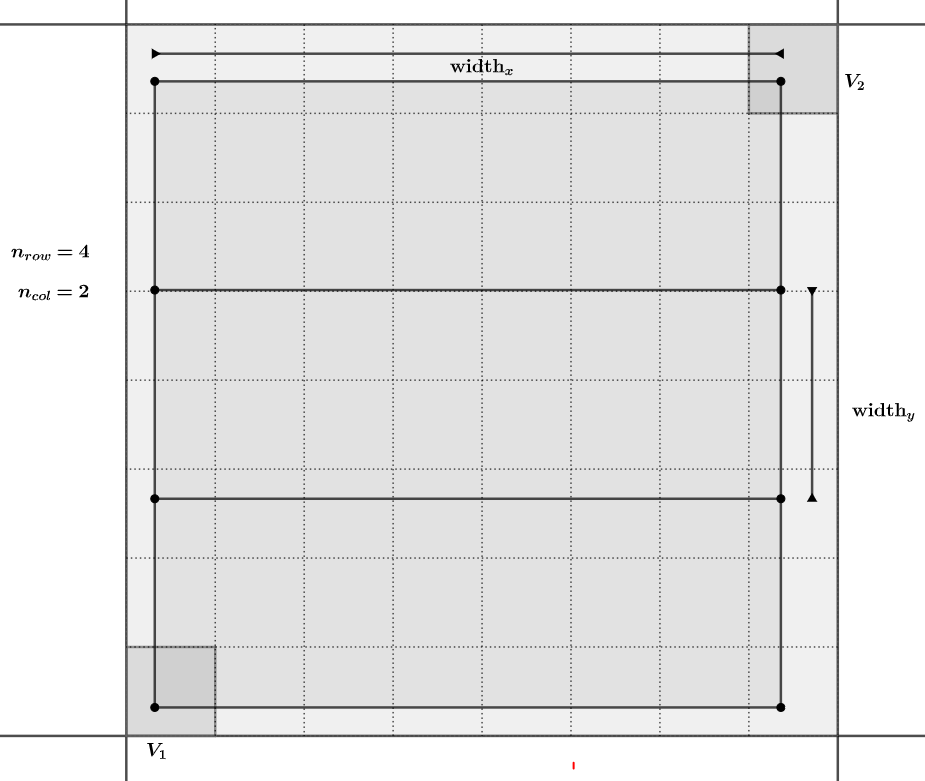
\includegraphics[width=1\linewidth]{Grid_generation.png}
% \end{center}
% \end{figure}
\noindent
In this section we discuss the experimental results obtained testing the formulations presented in Section \ref{Form} and the matheuristic procedure proposed in Section \ref{Math} on different sets of instances. In particular, we generated two sets of instances of the \AMD\xspace problem. The first one consists of targets, to be visited by the drone, that are represented by grid graphs, while the second one involves a different typology of targets, that is, Delaunay graphs. 
For both typologies we generated 5 instances of 10 graphs each, with different cardinality of the set of nodes. More precisely, each instance is composed of 3 graphs with 4 nodes, 3 graphs of 6 nodes, 3 graphs of 8 nodes and 1 graph of 10 nodes. Moreover, we assumed that the drone's speed is twice that of the mothership and that a percentage equal to $80\%$ of each target must be visited by the drone.\\
In order to locate in the space the 10 graphs of a single instance, we considered a square of side 100 units. Then we divided the original square in subsquares of side 5 and we randomly selected among them the locations for the ten target graphs of the instance. The generation procedure of the single graph in a selected square, depends on the graph typology.
As regards grid graphs, the single subsquare, like the one represented in Figure \ref{fig:fig1}, is further partitioned in subsquares of side $\frac{5}{n}$ where $n$ is the cardinality of the set of nodes of the graph to build. Two opposite corner subsquares have been considered (like $V_1$ and $V_2$ in Figure \ref{fig:fig1}) and one point inside each of them was randomly selected (black points in the subsquares $V_1$ and $V_2$ in Figure \ref{fig:fig1}). Then, a rectangle whose diagonal joins these two points has been built (the black dotted one in Figure \ref{fig:fig1}). A grid of $n$ points has been identified by locating $\frac{n}{m}$ 
%\CV{here we have n/m rows and m columns selected randomly in the set of divisors of the number of points of the graph)}
equally spaced points on the two sides square (the red ones and the two original points in black in Figure \ref{fig:fig1}), where $m$ is randomly selected in the set of divisors of the number of points of the graph. The links of the graphs connect each point to its adjacent ones lying on the same side and with the one located on the opposite side of the square.  Let $width_x$ and $width_y$ be the lengths  of these edges as show in Figure \ref{fig:fig1}. In order to perturb the coordinates of these points, we randomly added a value, ranging between $-\frac{width_x}{3}$ and $\frac{width_x}{3}$ to the $x$ coordinate and between $-\frac{width_y}{3}$ and $\frac{width_y}{3}$ to the $y$ coordinate, always imposing that the perturbed point still belongs to the square. The resulting grid graph is obtained connecting the same pairs of points but with perturbed coordinates (blue graph in Figure \ref{fig:fig1}). \\
As regards the instances related to Delaunay graphs, we adopted the same procedure as for the grid ones, for selecting their locations in the space. Then, for each randomly selected subsquare, given the set of $n$ nodes of the graph to be generated, a Delaunay triangulation of them is computed by using the Python class scipy.spatial.Delaunay (see \cite{art:Virtanen2020} for further details).





\begin{figure}[h!]
\begin{center}
 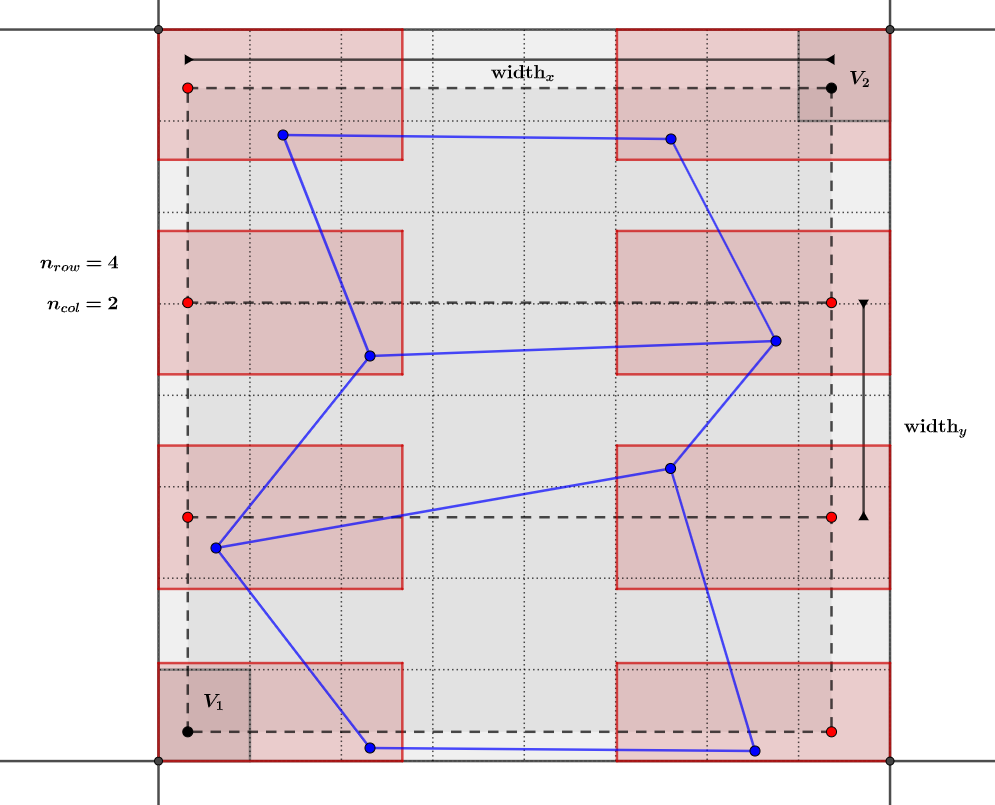
\includegraphics[width=0.6\linewidth]{Grid_generation_2.png}
\end{center}
\caption{Example of generation of a grid graph}
\label{fig:fig1}
\end{figure}
 
 
\noindent
We run the three formulations proposed in Section \ref{Form} for the \AMD\xspace problem (Stages, MTZ and SEC) with two different commercial solvers, Cplex 12.8 and Gurobi 9.03, called by means of Python, by setting a time limit for each run equal to 3600 sec.
In Table \ref{table:tab1} we reported the results obtained, in terms of average, minimum and maximum percentage with both solvers, on the instances consisting of grid graphs. First, we can observe that Gurobi has better performances with respect to Cplex for all the instances. Moreover, for this set of instances, the SEC formulation is the best one among the three proposed, as the associated average gap is equal to 0.61\% and also the minimum and the maximum percentage gap are smaller than the ones associated with the Stages and the MTZ formulations.\\

 
\renewcommand{\arraystretch}{0.7}
\begin{table}[!h]
\caption{Comparison between formulations for grid instances}
\centering
\footnotesize
\begin{tabular}{c | c c | c c | c c}
\hline\hline
\textbf{Gap \%} & \multicolumn{2}{c}{Average} &  \multicolumn{2}{c}{Min} &  \multicolumn{2}{c}{Max} \\
 % \hline
\textbf{Solver} &Cplex &Gurobi &Cplex &Gurobi  &Cplex &Gurobi \\
\hline
\textbf{Formulation} & & & & & &\\
Stages & 0,87 &	0,87 &	0,85 &	0,84 &	0,88 &	0,88\\
MTZ	 & 0,66 &	0,62 &	0,59 &	0,58 &	0,72 &	0,65\\
SEC	& 0,65 &	0,61 &	0,59 &	0,57 &	0,70 &	0,64\\
    \hline
\end{tabular}
\label{table:tab1}
\end{table}


\noindent
Similarly, Table \ref{table:tab2} summarizes the results obtained on the instances with Delaunay graphs. Also in this case the Gurobi performances are better than Cplex. However, among the three formulations, the MTZ one provides the best results in terms of average and maximum percentage gap.



\renewcommand{\arraystretch}{0.7}
\begin{table}[!h]
\caption{Comparison between formulations for Delauney instances}
\centering
\footnotesize
\begin{tabular}{c | c c | c c | c c}
\hline\hline
\textbf{Gap \%} & \multicolumn{2}{c}{Average} &  \multicolumn{2}{c}{Min} &  \multicolumn{2}{c}{Max} \\
 % \hline
\textbf{Solver} &Cplex &Gurobi &Cplex &Gurobi  &Cplex &Gurobi \\
\hline
\textbf{Formulation} & & & & & &\\
Stages &	0,91 &	0,91 &	0,90 &	0,89 &	0,93 &	0,93\\
MTZ	& 0,78 &	0,74 &	0,74 &	0,70 &	0,82 &	0,79\\
SEC	& 0,77 &	0,75 &	0,73 &	0,69 &	0,82 &	0,81\\
    \hline
\end{tabular}
\label{table:tab2}
\end{table}


\noindent
In order to test the performances of the matheuristic proposed in Section \ref{Math}, we coded it in Python and we run it on the same sets of instances (Grid and Delaunay) on which the three formulations have been solved. Table \ref{table:tab3} reports for each instance, numbered from 0 to 4, distinguishing between Grid and Delauney, respectively, the best objective function provided by the best formulation, the objective function provided by the matheuristic and the associated CPU time. As already noticed from Table \ref{table:tab2}, for grid graph instances, SEC formulation has the best behaviour, with the exception of the instance number 3 for which the MTZ provides a smaller value of the objective function. As for the Delaunay graph instances, MTZ is the best formulation, but also in this case there is an exception on the instance number 2 for which SEC formulation returns a smaller value of the objective function.\\
The results show that the matheuristic returns a solution with value of the objective function that is higher than the one provided by the SEC formulation on grid instances. However, these values are smaller than the ones provided by the Stages and the MTZ formulations. Moreover, the saving in terms of resolution time is very significant as the maximum CPU time is less than 1 minute.  As regards the Delaunay instances, the matheuristic performances are even better, as it finds a solution that is better than the best one provided by the MTZ formulation and in a resolution time that is at most 28 minutes. 



\renewcommand{\arraystretch}{0.7}
\begin{table}[!h]
\caption{Heuristic performances}
\centering
\footnotesize
\begin{tabular}{c | c c c | c c c}
\hline
\textbf{\#}  & \multicolumn{3}{c}{\textbf{Grid}} &  \multicolumn{3}{c}{\textbf{Delauney}} \\
 % \hline
 &Best Obj & Obj Heuristic &CPU Time &Best Obj & Obj Heuristic & CPU Time \\
\hline
0 &	1087,87	& 1117,83 &	50,99 &	947,01 &	934,46 &	52,49\\
1 &	1100,38	& 1319,64 &	24,64 &	986,22 &	 938,68	& 72,73\\
2 &	1350,67	& 1126,35 &	46,06 &	888,48 &	865,66 &	1073,80\\
3 &	1218,66	& 1476,36 &	27,18 &	1249,69 &	1154,62 &	1703,33\\
4 &	1297,77	& 1424,37 &	40,91 &	1239,93	 & 1184,67 &	81,15\\
    \hline
\end{tabular}
\label{table:tab3}
\end{table}


\noindent
We performed a second set of experiments by observing that, even if there are small differences between the SEC and the MTZ formulations depending on the type of instances, their performances are comparable.
Thus, in the rest of the tests we focused on the MTZ formulation. We compared its performances, with or without providing the initial solution found by the matheuristic, on a set of larger instances. More precisely, we generated 20 instances with targets represented by grid graphs and 20 instances with targets represented by Delauney graphs. The instances of each typology are split in 4 groups of 5 instances each, consisting respectively of 5, 10, 15 and 20 targets to be visited.
In each instance the same percentage of graphs ($20\%$) has respectively 4, 6, 8, 10 and 12 nodes. 
Moreover, we assumed that the origin coincides with the destination in all instances and we randomly generated with uniform distribution between 0 and 1, two values representing the percentage of each edge and of each graph to be visited.
As regards the speeds, we set the speed of the drone three times the one of the mothership.
We run the MTZ formulation by adopting Gurobi, setting a time limit of 7200 sec. for each instance.
On the same instances also the matheuristic has been applied. Note that, in order to define a stopping rule for the exact resolution of the \AMD\xspace model within the matheuristic procedure (STEP 3 and STEP 4), we set the maximum number of solutions generated by the solver equal to five.
For each instance, the solution provided by the matheuristic has been then used to initialize the exact resolution of the MTZ formulation in order to try to speed up the resolution process.
Table \ref{table:tab4} shows the results of the comparison between the exact resolution of the formulation with and without initialization. In the first column, named List, we report the size of the instances in terms of number of targets to be visited (0, 1, 2 and 3 identifies instances respectively with 5, 10, 15 and 20 graphs).The second column refers to the two variants of the model, that is, a given percentage of each edge of the targets (e) or a given percentage of each target (g) must be visited by the drone. The other columns report respectively the average percentage gap of the solutions found within the time limit starting from the initial solution provided by the matheuristic, the average running time of the matheuristic and the average percentage gap of the solutions found within the time limit without initialization. These information are reported for both Grid and Delauney instances.

\renewcommand{\arraystretch}{0.7}
\begin{table}[!h]
\caption{Comparison between exact resolution with and without initialization}
\centering
\footnotesize
\begin{tabular}{c c | c c c | c c c}
\hline
 &  & \multicolumn{3}{c}{\textbf{Grid}} &  \multicolumn{3}{c}{\textbf{Delauney}} \\
\hline
 List &  $\%$  & $\%$ Gap (i) & Time$\_$h & $\%$ Gap (ni)  & $\%$ Gap (i) & Time$\_$h &  $\%$ Gap (ni)\\
\hline
\multirow{}{}{0} & e & 0.72 & 105.12 & 0.73 & 0.78 & 154.92 & 0.74\\
& g & 0.55 & 58.92 & 0.54 & 0.62 & 92.64 & 0.67\\
\hline
\multirow{}{}{1} & e & 0.76 & 241.99 & 0.76 & 0.80 & 314.69 & 0.79\\
& g & 0.71 & 182.61 & 0.70 & 0.74 & 353.04 & 0.75\\
\hline
\multirow{}{}{2} & e & 0.76 & 367.69 & 0.76 & 0.80 & 447.61 & 0.80 \\
& g & 0.71 & 326.49 & 0.72 & 0.76 & 429.16 & 0.76\\
\hline
\multirow{}{}{3} & e & 0.75 & 481.68 & 0.74 & 0.80 & 514.98 & 0.76^*\\
& g & 0.71 & 492.27 & 0.70 & 0.77 & 582.90 & 0.77\\
    \hline
\end{tabular}
\label{table:tab4}
\end{table}

\noindent
From Table \ref{table:tab4} we can notice that in most of the cases the average gaps associated with the solution found within the time limit, with and without initialization by the solution found by the matheuristic, are the same or very close (note that in the last column the $*$ indicates that only one instance has been solved within the time limit).
As regards the running time of the matheuristic, we can see also from the boxplots in Figure \ref{fig:1}, that it increases with the number of targets to be visited both for Grid and Delaunay instances. Considering the model variants based on the minimum percentage of each edge or each graph to visit, we can observe that for Grid instances the average running time of the model imposing a minimum percentage of each edge to be visited, is greater than the one associated with the other variant, with the exception of the instances of biggest size (List=3). \\
\noindent
The boxplots in Figure \ref{fig:2} represent the percentage gap of the solution provided by the matheuristic with respect to the one provided by the exact resolution of the MTZ model within the time limit, with initialization by the solution found by the matheuristic. From them we can notice that the gap increases with the size both for Grid and Delaunay instances but it is always less than 0.5$\%$.  
Figure \ref{fig:3} shows the percentage gap of the solution provided by the exact resolution of the MTZ formulation within the time limit without the initialization, with respect to the one found with the initialization. This gap is very close to 0 both for Grid and Delaunay instances. Only for the biggest size we observe values ranging between 0.1$\%$ and 0.6$\%$. These observations suggest that, even if the initialization of the model by the solution provided by the matheuristic does not speed up the convergence to the optimal solution, the matheuristic provides solutions of very good quality. Indeed, it generates in less than 10 minutes solutions that are very close to the ones provided by the model within 2 hours.\\


\begin{figure}[htp]% [H] is so declass\'e!
\centering
\begin{minipage}{0.45\textwidth}
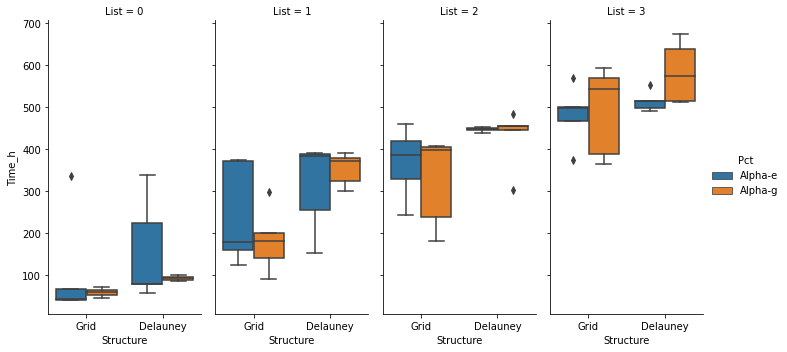
\includegraphics[width=\textwidth]{time_h.png}
\caption{Matheuristic running time}
\label{fig:1}
\end{minipage}\hfill
\begin{minipage}{0.45\textwidth}
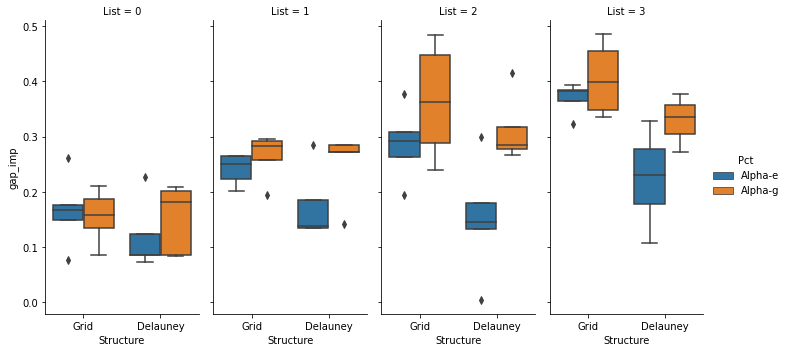
\includegraphics[width=\textwidth]{improved_gap.png}
\caption{Matheuristic improved gap}
\label{fig:2}
\end{minipage}\par
\vskip\floatsep% normal separation between figures
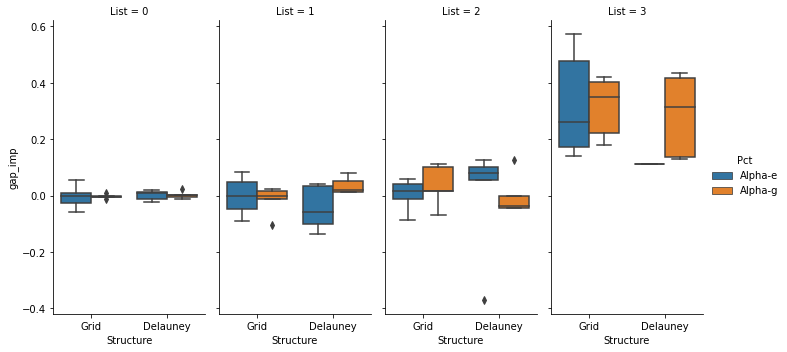
\includegraphics[width=0.45\textwidth]{differencewithwithout.png}
\caption{Improved gap of MTZ formulation with and without initialization}
\label{fig:3}
\end{figure}



\noindent
As regards the \NMD \xspace problem, we generated three sets of instances with targets represented by grid graphs considering different structures of the polygonal network where the mothership can move.
In particular, we defined a first set of instances where the mothership network is represented by a graph of 6 nodes with a tree structure with origin of the path of the base vehicle different from the destination.
A second set of instances involving a mothership network consisting in a complete graph of 4 vertices with origin of the path of the base vehicle different from the destination.  
A third set of instances characterized by star graphs of 7 nodes representing the mothership network, where the origin coincides with the destination and it is located at the centre of the star. We generated 10 instances for each of these three classes, 5 of them with 5 targets and 5 with 10 targets to be visited. 
Moreover, as for the \AMD\xspace, for each of these 10 instances we randomly generated two values representing the percentage of each edge and of each graph that must be visited by the drone.
We run on these sets of instances both Stages and MTZ formulations. Table \ref{table:tab5} summarizes the results obtained comparing them. The first column identifies the size of the instances, similarly to Table \ref{table:tab4}, (0 for instances with 5 targets and 1 for instances with 10 targets).
The second column distinguishes between minimum percentage of each edge (e) or of each graph (g) to be visited by the drone.
The remaining columns refer to the three different class  of instances described above (1 for the networks with a tree structure, 2 for complete networks and 3 for start networks).
For each of these sets of instances the average percentage gap of the solutions found within the time limit of 7200 sec. by the two formulations (Stages and MTZ) is reported.


\renewcommand{\arraystretch}{0.7}
\begin{table}[!h]
\caption{Comparison between formulations of \NMD}
\centering
\footnotesize
\begin{tabular}{c c | c c | c c | c c}
\hline
 & Net Struct  & \multicolumn{2}{c}{1} &  \multicolumn{2}{c}{2}  & \multicolumn{2}{c}{3}\\
\hline
List & $\%$ &  Stages  & MTZ & Stages & MTZ  & Stages & MTZ\\
\hline
\multirow{}{}{0} & e & 0.89 & 0.33 & 0.88 & 0.24 & 0.87 & 0.39\\
& g & 0.86 & 0.29 & 0.89 & 0.18 & 0.90 & 0.42\\
\hline
\multirow{}{}{1} & e & 0.92 & 0.43 & 0.92 & 0.33 & 0.92 & 0.46\\
& g & 0.91 & 0.36 & 0.92 & 0.23 & 0.92 & 0.39\\
\hline
\end{tabular}
\label{table:tab5}
\end{table}

\noindent
We can observe that for each class of instances and model variants, based on the percentage of each edge or each graph to be visited, the MTZ formulation performs better than the Stages one. In all the cases the percentage average gap associated with the MTZ formulation is one third or half of that associated with the Stages formulation. For this reason, in the following tests, related to the comparison between the exact resolution of the \NMD\xspace  model with and without the initialization by the solution found by the matheuristic, we focused only on the MTZ formulation.\\
Table \ref{table:tab6} summarizes the results of this comparison distinguishing again between the different network structures (columns labelled 1, 2 and 3), the different size (rows labelled 0 and 1) characterizing the instances and model variants (minimum percentage of each edge (e) or each graph (g) to be visited). For each combination of network structure, size and model variant we reported the average percentage gap with initialization ($\%$ Gap (i)), the solution time of the matheuristic (T$\_$h) and the average percentage gap without initialization by the solution found by the matheuristic ($\%$ Gap (ni))

\renewcommand{\arraystretch}{0.8}
\begin{table}[!h]
\caption{Comparison between exact resolution with and without initialization of \NMD}
\centering
\tiny
\begin{tabular}{c c | c c c | c c c | c c c}
\hline
 & Net Struct  & \multicolumn{3}{c}{1} &  \multicolumn{3}{c}{2}  & \multicolumn{3}{c}{3}\\
\hline
List &  $\%$  & $\%$ Gap (i) & T$\_$h & $\%$ Gap (ni)  & $\%$ Gap (i) & T$\_$h &  $\%$ Gap (ni) & $\%$ Gap (i) & T$\_$h &  $\%$ Gap (ni)\\
\hline
\multirow{}{}{0} & e & 0.32 & 109.96 & 0.33 & 0.24 & 207 & 0.24 & 0.39 & 177.57 & 0.39\\
& g & 0.30 & 110.92 & 0.29 & 0.18 & 163.36 & 0.18 & 0.45 & 149.68 & 0.42\\
\hline
\multirow{}{}{1} & e & 0.48 & 1030.64 & 0.43 & 0.39 & 802.3 & 0.33 & 0.53 & 770.05 & 0.46\\
& g & 0.33 & 479.36 & 0.36 & 0.35 & 639.09 & 0.23 & 0.42 & 689.51 & 0.39\\
\hline
\end{tabular}
\label{table:tab6}
\end{table}

\noindent
We can observe that, similarly to the \AMD\xspace problem, the average gaps associated with the solution found within the time limit, with and without initialization by the solution found by the matheuristic, are very close. Considering the average running time we can notice that the \NMD\xspace  problem is more challanging to be solved with respect to the \AMD. It increases very fast with the size of the instances especially for the case in which the network where the mothership moves has a tree structure. Moreover, as for the Grid instances in the continuous case, the model variant imposing a minimum percentage of each edge to be visited takes more time to be solved.

\begin{figure}
\centering
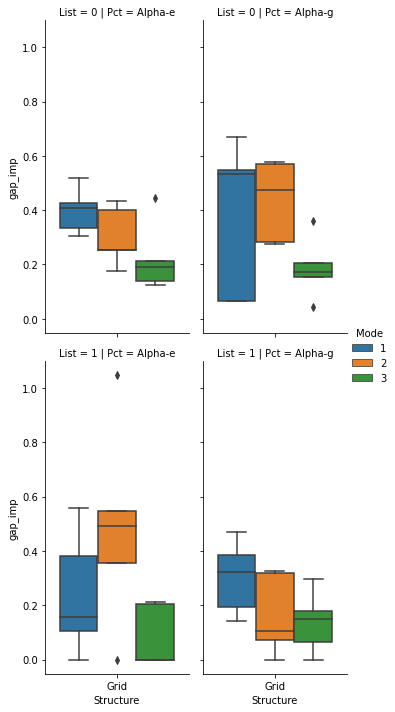
\includegraphics[width=5cm]{improved_gap_ND.png}
\caption{Matheuristic improved gap for \NMD}
\label{fig:4}
\end{figure}
\noindent
The boxplots showed in Figure \ref{fig:4} report the percentage gap of the solution provided by the matheuristic with respect to the one provided by the exact resolution of the MTZ model within the time limit, with initialization by the solution found by the matheuristic.
We can notice that, excluding the outliers, this gap ranges between 0$\%$ and 0.7$\%$ and its lowest values are observed for the instances in which the network where the mothership moves has a star structure (green boxplots). 
From the previous observations, similarly to the \AMD, we can conclude that the behaviour of the matheuristic is very good in terms of quality of the solutions provided, even if the initialization of the MTZ model does not help in speeding up the convergence to the optimal solution. 



\section{Concluding remarks}
\noindent
This papers has analyzed the coordination problem that arises between a mothership vehicle and a drone that must adjust their routes to minimize travel distances while visiting a set of targets modeled by graphs. We have presented exact formulations for different versions of the problem depending on the constraints imposed to the mothership movement (free on a continuous space or on a given network). Our computational results show that the considered problem is rather hard and only small to medium size problems can be  solved to optimality. Additionally, we have proposed a matheuristic algorithm, applicable to all the versions of the problem with minimum changes, that provides acceptable feasible solutions in short computing time;  so that it is a good alternative to the exact methods.\\
\noindent
Further research in this topic includes the coordination of the operations of several drones with a mothership, the possibility of visiting more than one target per operation and combinations of both cases. These problems being very interesting are beyond the scope of this paper and will be the focus of a follow up paper.








% \input{extensions}
\section*{Acknowledgements}
\noindent
This research has been partially supported by Spanish Ministry of Education and Science/FEDER grant number  MTM2016-74983-C02-(01-02), projects FEDER-US-1256951, CEI-3-FQM331 and  \textit{NetmeetData}: Ayudas Fundaci\'on BBVA a equipos de investigaci\'on cient\'ifica 2019, and by University of Rome, Sapienza grant number: RM11916B7F962975.
%\section{Introduction}

% \bibliographystyle{apa}

\bibliographystyle{apalike}
% \printbibliography
\section*{References}
\bibliography{bibliography2}


\end{document}
